\documentclass[journal]{IEEEtran}
\usepackage[T1]{fontenc}
\usepackage{newtxtext,newtxmath}
\usepackage{amsmath}
\usepackage{graphicx}
\usepackage{booktabs}
\usepackage{multirow}
\usepackage{array}
\usepackage{siunitx}
\usepackage{xcolor}
\usepackage{tikz}
\usetikzlibrary{positioning,arrows.meta,calc,fit,backgrounds}
\usepackage{placeins}
\usepackage{float}
\usepackage{dblfloatfix}
\usepackage[hidelinks]{hyperref}
\graphicspath{{figures/}}
\sisetup{group-minimum-digits=4}

% abstract and index-terms headings end with a colon
\makeatletter
\def\abstract{\normalfont\@IEEEabskeysecsize\bfseries\textit{\abstractname}:\ \relax\@IEEEgobbleleadPARNLSP}
\def\IEEEkeywords{\vspace{0.4\baselineskip}\normalfont\@IEEEabskeysecsize\bfseries\textit{\IEEEkeywordsname}:\ \relax\@IEEEgobbleleadPARNLSP}
\makeatother

\newcommand{\ugm}{\si{\micro\gram\per\cubic\metre}}
\newcommand{\PM}{PM\textsubscript{2.5}}
\definecolor{cres}{HTML}{2A78D6}
\definecolor{cafno}{HTML}{EB6834}
\definecolor{cgray}{HTML}{6B6B66}
\definecolor{cphys}{HTML}{1BAF7A}

% allow more floats per page so tables and figures stay near their text
\renewcommand{\topfraction}{0.9}
\renewcommand{\bottomfraction}{0.6}
\renewcommand{\textfraction}{0.08}
\renewcommand{\floatpagefraction}{0.8}
\renewcommand{\dbltopfraction}{0.9}
\renewcommand{\dblfloatpagefraction}{0.8}
\setcounter{topnumber}{3}
\setcounter{bottomnumber}{2}
\setcounter{totalnumber}{5}
\setcounter{dbltopnumber}{3}
% float-only pages: stack floats from the top instead of spreading them over the page
\makeatletter
\setlength{\@fptop}{0pt}\setlength{\@fpsep}{14pt}\setlength{\@fpbot}{0pt plus 1fil}
\setlength{\@dblfptop}{0pt}\setlength{\@dblfpsep}{14pt}\setlength{\@dblfpbot}{0pt plus 1fil}
\makeatother

\begin{document}

\title{Pipeline Over Backbone: A Controlled Study of Deep Networks for \PM{} Forecasting over India}

\author{\textbf{Vetriselvan~R}\\
Rishihood University\\
\texttt{vetriselvan.radhakrishnan2024@nst.rishihood.edu.in}}

\markboth{}{}
\hypersetup{pdftitle={Pipeline Over Backbone: A Controlled Study of Deep Networks for PM2.5 Forecasting over India}, pdfauthor={Vetriselvan R}}

\maketitle

\begin{abstract}
Deep networks for gridded air-quality forecasting are usually compared with their inputs, validation, loss and post-processing changed along with the architecture, so a gain cannot be credited to the network. We separate the two for 16-hour \PM{} forecasting over India on a $140\times124$ grid of WRF-Chem fields. We build one physics-informed, leak-free pipeline, with ventilation and advection channels, a log-space persistence residual and a loss matched to the evaluation metric, and train five networks inside it, with decision rules fixed before each stage and up to five seeds. Moving the same network into this pipeline raised its held-out test score 6 to 8 times more than choosing the better of the two best networks. Inside the fixed pipeline, a U-Net with a convolutional GRU over lead time (ResGRU-UNet) beats an adaptive Fourier neural operator (AFNO V4) on all 25 seed pairs, on both parts of the test set and at every lead hour, with 31.8\% lower RMSE than persistence (validation $R^2$ 0.892 against 0.874). Validation and test rank 25 forecasts alike (Spearman 0.93). Single-change ablations do not explain the gap, the ranking of the weaker networks changes with the metric, and a gradient-boosted correction lowers RMSE but not the benchmark score.
\end{abstract}

\begin{IEEEkeywords}
air quality forecasting, \PM, neural operators, convolutional recurrent networks, controlled comparison, spatio-temporal deep learning
\end{IEEEkeywords}

\section{Introduction}
\label{sec:intro}
\IEEEPARstart{F}{ine} particulate matter (\PM) is the largest environmental health risk in India: air pollution was linked to an estimated 1.67 million deaths there in 2019 \cite{pandey2021}. Country-wide forecasts usually come from chemistry transport models such as WRF-Chem \cite{grell2005}, which couple weather, emissions, chemistry and transport and are expensive to run. A deep network that learns to step such a model forward from its recent fields could forecast at a small fraction of the cost.

Forecasting \PM{} over a whole country is a large spatio-temporal problem: here 17{,}360 grid cells, 16 lead hours, and weather fields that carry pollution across the map. Two families of deep networks suit gridded forecasting. Fourier neural operators mix the whole map at once in the frequency domain \cite{li2021fno,guibas2022afno}. Convolutional-recurrent networks pass local information step by step \cite{shi2015convlstm,ballas2016convgru}. Published comparisons between them usually change the inputs, validation, loss and post-processing along with the network, so a difference in score cannot be credited to the network alone. In image classification, a better training recipe closed much of the reported gap between older and newer architectures \cite{wightman2021,bello2021,liu2022convnext}, and in long-horizon forecasting one-layer linear models beat Transformers \cite{zeng2023}. Whether the same holds for gridded air-quality forecasting has, to our knowledge, not been tested.

The two effects are hard to separate in practice. A network is usually developed together with its pipeline, and each new pipeline is tuned around the network it was built for, so a comparison with a network trained in an older pipeline mixes the two. Our own development followed this path (Appendix~\ref{sec:history}): over seven iterations the split, the episode masks, the inputs, the loss, the hour handling and the post-processing all changed together with the network, and at the end the question ``which network is better?'' had no clean answer.

In this paper we test the question directly. We fixed the pipeline that the seven iterations produced and trained five networks inside it, two Fourier neural operators and three convolutional-recurrent networks, changing nothing but the network. Decision rules were written down before each stage, and the finalists were run with 1, 2 and 5 seeds. Fig.~\ref{fig:teaser} shows the main result: moving a network into the improved pipeline raised its held-out test score by 0.025 to 0.031, while the best network beat the second best by 0.0036 at one seed and 0.0066 with the full recipe.

\begin{figure}[!t]
\centering
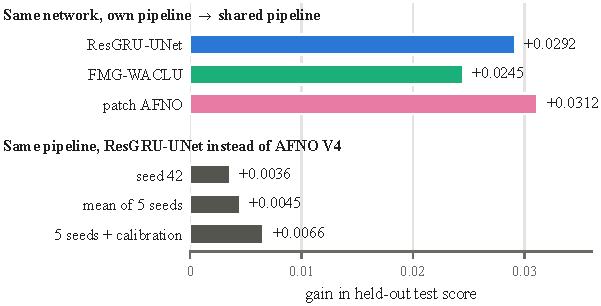
\includegraphics[width=\columnwidth]{fig_teaser.pdf}
\caption{Gain in held-out test score from moving each network from its own earlier pipeline into the shared pipeline (coloured; one seed, no ensemble or calibration; patch AFNO's gain includes a bug fix), against the gain from choosing ResGRU-UNet over AFNO V4 inside the shared pipeline (grey): at one seed, as the mean of five single seeds, and with five-seed ensembles and calibration.}
\label{fig:teaser}
\end{figure}

The study gives three findings. First, the pipeline matters more than the network: the same network gains 6 to 8 times more from the pipeline than from the choice between the two best networks. Second, inside one pipeline the convolutional-recurrent U-Net beats the neural operator on every seed pair, both parts of the test set, every lead hour, every month and every regression metric, and it is cheaper to run. Third, rankings and post-processing depend on the metric: the weaker networks reorder when the metric changes, and per-hour calibration raises the benchmark score while it worsens MAE, RMSE and $R^2$.

Our contributions are:
\begin{itemize}
\item a controlled comparison of five deep networks inside one fixed pipeline, with decision rules fixed before each stage, up to five seeds, a block bootstrap and a check that validation predicts the held-out test (Sections~\ref{sec:setup} and~\ref{sec:results});
\item evidence for the three findings, with ablations, training curves and breakdowns by lead hour, month, concentration and grid cell that test why the winner wins (Sections~\ref{sec:results} and~\ref{sec:analysis});
\item a physics-informed, leak-free pipeline with the reasoning behind each choice, regression metrics against three baselines, an out-of-fold test of an ML + DL hybrid, and the code and run records behind every number (Sections~\ref{sec:method}, \ref{sec:setup} and~\ref{sec:hybrid}).
\end{itemize}

Section~\ref{sec:related} reviews related work and Section~\ref{sec:data} the task, data and metric. Section~\ref{sec:method} describes the shared pipeline and the five networks, and Section~\ref{sec:setup} the validation, baselines, statistics and decision rules. Section~\ref{sec:results} reports the three findings and Section~\ref{sec:analysis} analyses where and why the winner wins, the hybrid, the linear baseline and the cost. Section~\ref{sec:discussion} discusses what the results mean, Section~\ref{sec:threats} the threats to validity, and Section~\ref{sec:conclusion} concludes. The appendices hold the data exploration, the development history, the architecture and run details, and the full tables.

\section{Related Work}
\label{sec:related}
\textbf{Chemistry transport and emulation.} WRF-Chem runs weather and chemistry together on one grid with one transport scheme \cite{grell2005}. For particulate matter over the Indian subcontinent, lightweight deep networks were reported to beat the Aurora foundation model at short horizons \cite{kushwaha2025}. CoNOAir, a complex neural operator, is reported to beat the Fourier neural operator for carbon monoxide in Indian cities \cite{bedi2025conoair}.

\textbf{Neural operators.} The Fourier neural operator (FNO) learns maps between function spaces with convolutions in Fourier space \cite{li2021fno}. The adaptive FNO (AFNO) replaces FNO's weight per mode with a small shared MLP over blocks of channels and a soft threshold that keeps the spectrum sparse \cite{guibas2022afno}. AFNO is the backbone of the FourCastNet global weather model \cite{pathak2022fourcastnet}, and AdaptFNO adds multiscale learning for climate fields \cite{dang2025adaptfno}.

\textbf{Convolutional-recurrent forecasting.} ConvLSTM replaced the matrix products of an LSTM with convolutions for precipitation nowcasting \cite{shi2015convlstm}; TrajGRU followed \cite{shi2017trajgru}, and the convolutional GRU is the gated-recurrent version \cite{ballas2016convgru}. U-Net's skip connections pass fine detail from encoder to decoder \cite{ronneberger2015unet}, and residual learning makes deep stacks easy to train \cite{he2016}. SimVP showed that a purely convolutional encoder, translator and decoder can match recurrent models \cite{gao2022simvp}. Shortcut recurrent-convolutional U-Nets were used for weather prediction \cite{leinonen2021}.

\textbf{Recipe or architecture.} Several studies found that the training recipe, not the architecture, explained much of a reported gain. A plain ResNet-50 trained with a modern procedure reached 80.4\% ImageNet top-1 accuracy \cite{wightman2021}; improved training and scaling made ResNets competitive with newer models \cite{bello2021}; a ResNet modernized step by step competed with vision Transformers \cite{liu2022convnext}; and one-layer linear models beat Transformer forecasters on nine long-horizon benchmarks \cite{zeng2023}. In language modelling, well-regularized standard LSTMs tuned at scale matched or beat newer recurrent models \cite{melis2018}, and a large study of generative adversarial networks found that most models reach similar scores with enough tuning and random restarts \cite{lucic2018}. We run the same kind of test for gridded air-quality forecasting, with the pipeline, not only the optimizer settings, held fixed.

\textbf{Evaluation.} A point forecast should be judged with a scoring function matched to what it is meant to estimate; a mismatched score can lead to badly wrong conclusions \cite{gneiting2011}. SMAPE is not symmetric in additive error \cite{goodwin1999}. Dependent data need blocked rather than random validation \cite{roberts2017}, information the model would not have at forecast time inflates scores \cite{kaufman2012}, and the block bootstrap resamples blocks of consecutive observations to keep their dependence \cite{kunsch1989}. Data sampling, initialization and hyperparameter choice can change benchmark results markedly, so these sources of variation should be randomized and reported \cite{bouthillier2021}. Persistence and seasonal naive are the standard forecasts to beat \cite{hyndman2021}, and ridge regression \cite{hoerl1970} is our classical model.

\textbf{Training.} We use AdamW \cite{loshchilov2019}, the one-cycle schedule \cite{smith2019}, GroupNorm \cite{wu2018}, weight averaging \cite{polyak1992} and deep ensembles \cite{lakshminarayanan2017}. For the hybrid we use LightGBM \cite{ke2017lightgbm}.

\section{Problem, Data and Metric}
\label{sec:data}
\subsection{Task}
Given the fields $\mathbf{X}_{t-9:t}$ of the last 10 hours, one network forecasts all 16 hours at once,
\begin{equation}
\hat{\mathbf{y}}_{t+h} = f_\theta(\mathbf{X}_{t-9:t})_h, \qquad h = 1,\dots,16,
\end{equation}
where each $\hat{\mathbf{y}}_{t+h}$ is a $140\times124$ map of \PM{} in \ugm. The task is a regression problem. A window spans 26 hours, 10 inputs and 16 targets.

\subsection{Data}
The data are WRF-Chem simulation fields released by the organizers of the ANRF AISEHack 2026 challenge (Theme 2, IIT Delhi) \cite{aisehack2026}. Training covers four months of 2016, one per season (April, July, October and December; 715 or 739 hours each), on a Mercator grid of $140\times124$ cells from 7.06 to 38.00$^\circ$N and 67.79 to 97.93$^\circ$E, about 25~km apart (27.1~km east to west at the southern edge and 21.5~km at the northern edge). Each hour has 16 fields: surface \PM{} (the target), eight weather fields and seven emission fields (Table~\ref{tab:fields}).

\begin{table}[!htb]
\centering
\caption{The 16 hourly fields of the data (units as released) and their use}
\label{tab:fields}
\setlength{\tabcolsep}{3pt}
\begin{tabular}{@{}ll>{\raggedright\arraybackslash}p{0.42\columnwidth}@{}}
\toprule
Field & Unit & Meaning and use \\
\midrule
\PM{} (cpm25) & \ugm & surface concentration; target and input \\
q2 & kg/kg & 2-m specific humidity; input \\
t2 & K & 2-m temperature; input \\
u10, v10 & m/s & 10-m zonal and meridional wind; input, advection, ventilation \\
swdown & W/m$^2$ & downward shortwave radiation; input, hour estimation \\
pblh & m & boundary-layer height; input, ventilation \\
psfc & Pa & surface pressure; input \\
rain & mm & rain in the hour; input (log) \\
7 emissions & & primary \PM, NH$_3$, SO$_2$, NO$_x$, two NMVOC fields, biogenic isoprene; not used (Section~\ref{sec:eda}) \\
\bottomrule
\end{tabular}
\end{table}

The test set is 218 windows of 10 hours from 2017; its answers are hidden and scored by the organizers' evaluation server. The server reports the score on two parts of the test set, a public part and a private part. Throughout the paper, ``test'' means the private part. The public part, which gave feedback during the early development iterations (Appendix~\ref{sec:history}), is reported alongside it where it adds evidence (Appendix~\ref{app:tests}, Tables~\ref{tab:seeds} and~\ref{tab:tests}).

\subsection{Episodes}
For each cell $i$, a robust STL decomposition \cite{cleveland1990} with a 24-hour period splits the month into trend, daily cycle and residual $r_{i,t}$. An hour is an episode when
\begin{equation}
r_{i,t} > 3\,\sigma_i \quad\text{and}\quad y_{i,t} > 1~\ugm,
\end{equation}
where $\sigma_i$ is the standard deviation of that cell's residuals. Episodes are 1.8\% of the validation values (1{,}082{,}178 of 59{,}440{,}640). They are defined on the truth, so a forecaster cannot know in advance which cells will be episodes; Section~\ref{sec:theory} shows why this matters.

\subsection{Benchmark Score}
\label{sec:score}
With $\mathrm{SMAPE}(p,y)=|p-y|/\bigl(\tfrac12(|p|+|y|)\bigr)$, let $G$ be the mean SMAPE over all cells and hours, $E$ its mean over episode cells, and $\rho$ the Pearson correlation of forecast and truth over episode cells, computed per hour and averaged. The benchmark score is
\begin{equation}
S = w_1\bigl(1-\tfrac{G}{2}\bigr) + w_2\,\tfrac{1+\rho}{2} + w_3\bigl(1-\tfrac{E}{2}\bigr).
\label{eq:score}
\end{equation}
The weights are not disclosed, so on validation we use $w_i=1/3$. Each term lies in $[0,1]$, and higher is better. $S$ is a composite of relative error and correlation, not an accuracy: two of its three terms see only the 1.8\% of values that are episodes, and none of them is on the raw scale of the concentration.

\subsection{What the Data Showed}
\label{sec:eda}
Table~\ref{tab:eda} lists what the exploration of the four training months showed and what each finding changed in the pipeline; Appendix~\ref{app:eda} gives the details. Three findings shaped the method most. The concentration is right-skewed (skewness 5.1, but 0.13 after the log), so the networks work in $\log(1+y)$. The field is persistent at short lead and loses that memory over the horizon (the lag-1 autocorrelation of $\log(1+y)$ is 0.978, and the standard deviation of its change grows from 0.101 after one hour to 0.505 after 16), so the networks predict the change from persistence and later hours carry more weight in the loss. Finally, the wind moves \PM{} about 10 cells in 16 hours, so a forecast needs a receptive field of that size, not the whole map.

\begin{table}[!htb]
\centering
\caption{What the data showed (training months) and what it changed}
\label{tab:eda}
\begin{tabular}{@{}>{\raggedright\arraybackslash}p{0.55\columnwidth}>{\raggedright\arraybackslash}p{0.37\columnwidth}@{}}
\toprule
Finding & What the model gets \\
\midrule
Right-skewed: December mean 59.1, median 23.7~\ugm & Work in $\log(1+y)$ \\
Lag-1 autocorrelation of $\log(1+y)$ is 0.978; the standard deviation of its change grows from 0.101 at 1 h to 0.505 at 16 h & Predict the change from persistence; weight later hours more \\
Mean 10-m wind 4.24~m/s: \PM{} moves about 10 cells in 16 h & Advection channel; a local receptive field suffices \\
Strong daily cycle (correlation 0.571 at 24 h); test windows carry no clock & Estimated hour; diurnal anomaly \\
Hotspots over the Indo-Gangetic Plain and the eastern coal belt; monthly means 15.4 (July) to 59.1 (December) & Per-cell normalization; static climatology \\
Episodes are about 2\% of cell-hours and are defined on the truth & Episode-weighted loss; calibration \\
Emission fields are tiny (April maxima $8\times10^{-9}$ to $7\times10^{-6}$) & Not used \\
\bottomrule
\end{tabular}
\end{table}

\section{Method: One Pipeline for Every Network}
\label{sec:method}
Fig.~\ref{fig:overview} shows the pipeline. Each part below was added to fix a problem that an earlier iteration exposed (Appendix~\ref{sec:history}), and each is shared by all five networks.

\begin{figure*}[!tb]
\centering
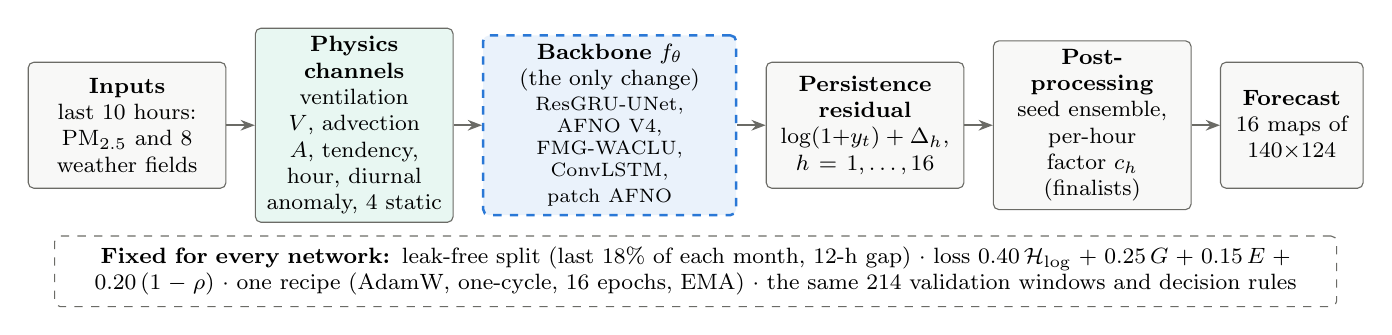
\begin{tikzpicture}[font=\footnotesize, node distance=3.6mm,
  b/.style={draw=cgray, rounded corners=2pt, align=center, minimum height=16mm, inner sep=3pt, text width=23mm, fill=cgray!5},
  arr/.style={-{Stealth[length=1.8mm]}, cgray, thick}]
\node[b] (in) {\textbf{Inputs}\\ last 10 hours:\\ \PM{} and 8\\ weather fields};
\node[b, fill=cphys!10, right=of in] (ph) {\textbf{Physics channels}\\ ventilation $V$, advection $A$, tendency, hour, diurnal anomaly, 4 static};
\node[b, fill=cres!10, draw=cres, dashed, line width=0.9pt, right=of ph, text width=30mm] (bb) {\textbf{Backbone} $f_\theta$\\ (the only change)\\[1pt] {\scriptsize ResGRU-UNet, AFNO V4,\\ FMG-WACLU, ConvLSTM,\\ patch AFNO}};
\node[b, right=of bb] (res) {\textbf{Persistence residual}\\ $\log(1{+}y_t)+\Delta_h$,\\ $h=1,\dots,16$};
\node[b, right=of res] (post) {\textbf{Post-processing}\\ seed ensemble,\\ per-hour factor $c_h$\\ (finalists)};
\node[b, right=of post, text width=16mm] (out) {\textbf{Forecast}\\ 16 maps of\\ $140{\times}124$};
\foreach \i/\j in {in/ph,ph/bb,bb/res,res/post,post/out} \draw[arr] (\i)--(\j);
\node[draw=cgray, dashed, rounded corners=2pt, anchor=north, align=center, text width=160mm, inner sep=4pt] at ($(in.west)!0.5!(out.east)+(0,-14mm)$) {\textbf{Fixed for every network:} leak-free split (last 18\% of each month, 12-h gap) $\cdot$ loss $0.40\,\mathcal{H}_{\log}+0.25\,G+0.15\,E+0.20\,(1-\rho)$ $\cdot$ one recipe (AdamW, one-cycle, 16 epochs, EMA) $\cdot$ the same 214 validation windows and decision rules};
\end{tikzpicture}
\caption{One pipeline for every network. Everything except the backbone (dashed blue) is fixed: inputs and physics channels, the residual output, the split, the loss, the training recipe and the evaluation. The study swaps only $f_\theta$. Seed ensembles and calibration are applied to the two finalists only.}
\label{fig:overview}
\end{figure*}

\subsection{Design Principles}
\label{sec:theory}
\textbf{Why log space.} For $p,y>0$ write $u=\log(p/y)$. Then
\begin{equation}
\mathrm{SMAPE}(p,y) = \frac{|p-y|}{(p+y)/2} = 2\,\bigl|\tanh(u/2)\bigr|,
\end{equation}
since $(p-y)/(p+y)=(e^u-1)/(e^u+1)$. SMAPE is therefore symmetric in the log ratio: twice too high and half too low cost the same, 0.667. Because SMAPE grows with $|u|$, the median minimizes the expected global SMAPE whenever $\log y$ is symmetric and unimodal around it. Predicting in $\log(1+y)$ therefore matches the metric, and the log transform also reduces the influence of the heavy right tail.

\textbf{Why a persistence residual.} Every network outputs a change $\Delta_h$ added to the last observed hour,
\begin{equation}
\hat{y}_{t+h} = \exp\bigl(\log(1+y_t) + \Delta_h\bigr) - 1,
\end{equation}
with the last layer set to zero at the start \cite{he2016}. An untrained network is therefore exactly persistence, which already scores 0.8515 on validation, and training only has to learn the departure from it.

\textbf{Why the episode terms reward upward shifts.} Episode cells are picked from the truth: where $y$ turned out high against its usual level. On those cells the truth is on average 50\% above persistence (mean $\log(y/\text{persistence})=+0.406$, against $-0.012$ over all cells). A forecast that cannot see the future noise therefore tends to score better on $E$ when it is shifted up; for persistence, the scale that maximizes the score rises with lead time from 1.00 to 1.30. Pearson $\rho$ does not change when a forecast is scaled, so a per-hour factor $c_h\ge1$ moves only the SMAPE terms. This is the basis of the calibration in Section~\ref{sec:training}, and it predicts the metric dependence of Section~\ref{sec:finding3}: a shift that helps $E$ on the 1.8\% of episode values must raise the error on the other 98.2\%.

\subsection{Physics-Informed Inputs}
\label{sec:physics}
Surface \PM{} changes through emission, transport, vertical mixing, chemistry and deposition. Three of these leave a mark in the available fields, and we compute each one as an input instead of leaving the network to find it. Table~\ref{tab:features} lists the 20 channels.

\textbf{Vertical mixing.} The boundary layer dilutes surface pollution in proportion to its depth and the wind that flushes it. Their product, the ventilation coefficient, measures how easily the air clears; its long decline over Indian cities goes with rising pollution potential \cite{iyer2013}. We add
\begin{equation}
V = \log\bigl(1+\mathrm{PBLH}\cdot\|\mathbf{u}_{10}\|\bigr)
\end{equation}
and the wind speed $\|\mathbf{u}_{10}\|$. Low values of $V$ indicate stagnant air, in which episodes tend to develop.

\textbf{Transport.} To first order a tracer follows $\partial_t C = -\mathbf{u}\cdot\nabla C$, so we add the advection of the log concentration,
\begin{equation}
A = -\bigl(u\,\partial_x + v\,\partial_y\bigr)\log(1+C),
\end{equation}
from centred differences. Earlier models used the same physics in other forms: ConvLSTM shifted the \PM{} map along the wind (a semi-Lagrangian step \cite{staniforth1991}), and FMG-WACLU added wind direction and divergence, since converging wind ($\nabla\cdot\mathbf{u}<0$) traps pollution.

\textbf{Time.} A window-local tendency $\Delta_t\log(1+C)$, divided by its per-cell spread, separates building from clearing episodes. The test windows carry no clock, so each window's start hour is estimated by matching its mean sunlight and temperature to hourly templates from training; this is exact for 60.7\% of validation windows and right within one hour for 97.7\%, and validation uses the estimate exactly as the test does. The hour enters as $(\sin,\cos)$, with the departure of $\log(1+C)$ from the cell's usual value at that hour, which mirrors the STL residual that defines an episode.

\textbf{Normalization.} \PM{} and rain are log-transformed; every channel is standardized per cell with training-period statistics, with a floor on the standard deviation and clipping at $\pm10$.

\begin{table}[!htb]
\centering
\caption{The 20 input channels in four groups}
\label{tab:features}
\begin{tabular}{@{}lrp{0.6\columnwidth}@{}}
\toprule
Group & $n$ & Channels \\
\midrule
Weather & 9 & $\log(1+\text{\PM})$, humidity, temperature, $u_{10}$, $v_{10}$, PBLH, pressure, shortwave radiation, $\log(1+\text{rain})$ \\
Physics & 3 & wind speed, ventilation $V$, advection $A$ \\
Time & 4 & tendency, hour $\sin$ and $\cos$, diurnal anomaly \\
Static & 4 & latitude, longitude, cell \PM{} climatology, cell STL residual spread \\
\bottomrule
\end{tabular}
\end{table}

\subsection{Five Backbones}
\label{sec:arch}
Table~\ref{tab:models} lists the five networks, and Appendix~\ref{app:arch} gives their layers. All read the same 20 channels and all output the residual of Section~\ref{sec:theory}. Each was ported from its original code; with the original input width and the same weights, each port reproduces the original output exactly (for ConvLSTM, with its season input, which these data lack, set to identity). A bug in the original patch AFNO, which dropped the imaginary half of every filtered spectrum, was fixed. Fig.~\ref{fig:arch} shows the two finalists.

\begin{table}[!htb]
\centering
\caption{The five networks (study versions, 20 input channels)}
\label{tab:models}
\setlength{\tabcolsep}{3pt}
\begin{tabular}{@{}lrp{0.58\columnwidth}@{}}
\toprule
Network & Params & Design and inductive bias \\
\midrule
ResGRU-UNet & 7.12M & all 10 hours stacked as 200 channels; conv U-Net; ConvGRU unrolled over the 16 lead hours \\
AFNO V4 & 6.98M & per-hour conv encoder; AFNO blocks at two scales; temporal translator; U-Net decoder \\
FMG-WACLU & 3.45M & ConvLSTM U-Net with wind physics and a gate from forecast weather \\
patch AFNO & 5.71M & $4\times4$ patches, AFNO blocks, linear unpatchify \\
ConvLSTM & 19.0M & ConvLSTM over the inputs, spectral block, wind-shift advection \\
\bottomrule
\end{tabular}
\end{table}

\begin{figure*}[!tb]
\centering
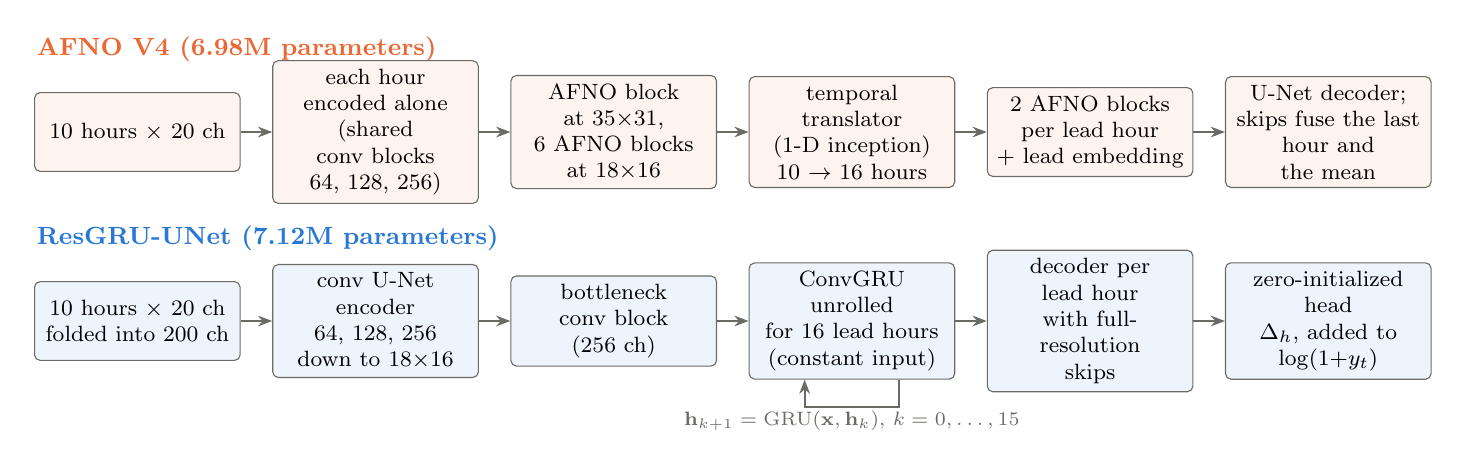
\begin{tikzpicture}[font=\footnotesize, node distance=4mm,
  b/.style={draw=cgray, rounded corners=2pt, align=center, minimum height=10mm, inner sep=3pt, text width=24mm},
  arr/.style={-{Stealth[length=1.8mm]}, cgray, thick}]
\node[font=\small\bfseries, text=cafno, anchor=west] at (-1.4,1.05) {AFNO V4 (6.98M parameters)};
\node[b, fill=cafno!8] (a0) at (0,0) {10 hours $\times$ 20 ch};
\node[b, fill=cafno!8, right=of a0] (a1) {each hour encoded alone\\ (shared conv blocks\\ 64, 128, 256)};
\node[b, fill=cafno!8, right=of a1] (a2) {AFNO block at $35{\times}31$,\\ 6 AFNO blocks\\ at $18{\times}16$};
\node[b, fill=cafno!8, right=of a2] (a3) {temporal translator\\ (1-D inception)\\ 10 $\to$ 16 hours};
\node[b, fill=cafno!8, right=of a3] (a4) {2 AFNO blocks\\ per lead hour\\ + lead embedding};
\node[b, fill=cafno!8, right=of a4] (a5) {U-Net decoder;\\ skips fuse the last\\ hour and the mean};
\foreach \i/\j in {a0/a1,a1/a2,a2/a3,a3/a4,a4/a5} \draw[arr] (\i)--(\j);
\node[font=\small\bfseries, text=cres, anchor=west] at (-1.4,-1.35) {ResGRU-UNet (7.12M parameters)};
\node[b, fill=cres!8] (r0) at (0,-2.4) {10 hours $\times$ 20 ch\\ folded into 200 ch};
\node[b, fill=cres!8, right=of r0] (r1) {conv U-Net encoder\\ 64, 128, 256\\ down to $18{\times}16$};
\node[b, fill=cres!8, right=of r1] (r2) {bottleneck\\ conv block\\ (256 ch)};
\node[b, fill=cres!8, right=of r2] (r3) {ConvGRU unrolled\\ for 16 lead hours\\ (constant input)};
\node[b, fill=cres!8, right=of r3] (r4) {decoder per lead hour\\ with full-resolution\\ skips};
\node[b, fill=cres!8, right=of r4] (r5) {zero-initialized head\\ $\Delta_h$, added to\\ $\log(1{+}y_t)$};
\foreach \i/\j in {r0/r1,r1/r2,r2/r3,r3/r4,r4/r5} \draw[arr] (\i)--(\j);
\draw[arr] ([xshift=6mm]r3.south) -- ++(0,-3.5mm) -- ([xshift=-6mm,yshift=-3.5mm]r3.south) -- ([xshift=-6mm]r3.south);
\node[below, font=\scriptsize, text=cgray, inner sep=1pt] at ([yshift=-3.6mm]r3.south) {$\mathbf{h}_{k+1}=\mathrm{GRU}(\mathbf{x},\mathbf{h}_k)$, $k=0,\dots,15$};
\end{tikzpicture}
\caption{The two finalists. AFNO V4 encodes each input hour separately and mixes the sequence in a coarse spectral bottleneck; its skip connections keep only the last hour and the mean of the 10 hours. ResGRU-UNet stacks all hours as channels in its first convolution and steps a convolutional GRU through the 16 lead hours. Both output the change $\Delta_h$ from persistence.}
\label{fig:arch}
\end{figure*}

\textbf{AFNO block.} Let $\hat{\mathbf{z}}=\mathrm{FFT}_2(\mathbf{z})$ be the orthonormal 2-D real Fourier transform of a feature map whose channels are split into $b=8$ blocks. At every Fourier mode, each block passes the same small complex MLP, then a soft threshold $S_\lambda$:
\begin{equation}
\mathcal{A}(\mathbf{z}) = \mathbf{z} + \mathrm{FFT}_2^{-1}\Bigl(S_\lambda\bigl(W_2\,\mathrm{ReLU}(W_1\hat{\mathbf{z}}+\mathbf{b}_1)+\mathbf{b}_2\bigr)\Bigr),
\end{equation}
with $\lambda=0.01$ and the ReLU applied to the real and imaginary parts separately \cite{guibas2022afno}. An AFNO block computes $\mathbf{x}\leftarrow\mathbf{x}+\mathcal{A}(\mathrm{GN}(\mathbf{x}))$, then $\mathbf{x}\leftarrow\mathbf{x}+\mathrm{MLP}(\mathrm{GN}(\mathbf{x}))$ with a $1\times1$ MLP of width $2d$ and GroupNorm GN. Every block sees the whole map, and the FFT treats opposite edges as neighbours.

\textbf{ConvGRU.} The bottleneck feature $\mathbf{x}$ is fed at every lead hour $k$ and a hidden state $\mathbf{h}_k$ is updated with $3\times3$ convolutions $*$ \cite{ballas2016convgru}:
\begin{align}
[\mathbf{r},\mathbf{u}] &= \sigma\bigl(W_g * [\mathbf{x},\mathbf{h}_k]\bigr), \\
\tilde{\mathbf{h}} &= \tanh\bigl(W_c * [\mathbf{x},\mathbf{r}\odot\mathbf{h}_k]\bigr), \\
\mathbf{h}_{k+1} &= (1-\mathbf{u})\odot\mathbf{h}_k + \mathbf{u}\odot\tilde{\mathbf{h}},
\end{align}
starting from $\mathbf{h}_0=\mathbf{x}$, with GroupNorm inside each gate. The recurrence runs over lead time, not over the input hours: the inputs enter once, through the stacked channels, and each $\mathbf{h}_{k}$ is decoded with the encoder's skips into the change for lead hour $k$.

\textbf{Other networks.} FMG-WACLU is a ConvLSTM U-Net that adds wind speed, direction and divergence and gates its features with weather rolled forward by a second ConvLSTM. ConvLSTM reads the 10 input hours recurrently at full resolution, adds an FNO-style spectral block, and shifts the \PM{} map along the wind; 88\% of its 19.0M parameters sit in the two spectral blocks of its bottleneck. Patch AFNO cuts the map into $4\times4$ patches, mixes them with AFNO blocks and maps each patch back with one linear layer.

\subsection{Training, Regularization and Calibration}
\label{sec:training}
\textbf{Loss.} Training minimizes a loss matched to the score,
\begin{equation}
\mathcal{L} = 0.40\,\mathcal{H}_{\log} + 0.25\,G + 0.15\,E + 0.20\,(1-\rho),
\end{equation}
where $\mathcal{H}_{\log}$ is the Huber loss on $\log(1+y)$ with episode cells weighted by 6. Lead hours are weighted linearly from 0.7 to 1.3 in $\mathcal{H}_{\log}$ and $G$, because errors grow with lead time while the score weights all hours equally. In the loss, $G$ and $E$ add 0.1 to the SMAPE denominator for stable gradients.

\textbf{Optimization.} AdamW \cite{loshchilov2019} with learning rate $2.5\times10^{-4}$ and weight decay $10^{-4}$, a one-cycle schedule \cite{smith2019}, 16 epochs, effective batch 4, mixed precision and gradient clipping at 1.0. One run takes about 51 minutes (ResGRU-UNet) or 90 minutes (AFNO V4) on one NVIDIA T4; Appendix~\ref{app:runs} lists every run.

\textbf{Regularization.} The networks have 3 to 19 million parameters but see only 2{,}257 training windows from four months, so we regularize them in several ways:
\begin{itemize}
\item channel dropout ($p=0.1$) in every convolution block of ResGRU-UNet and AFNO V4 and in AFNO V4's MLPs; ConvLSTM uses dropout 0.25 and stochastic depth 0.15;
\item decoupled weight decay $10^{-4}$;
\item an exponential moving average of the weights (decay 0.999) \cite{polyak1992}, which is the model we evaluate;
\item selection of the best epoch by the validation score, which acts as early stopping;
\item gradient clipping, per-cell standardization with floors, and input clipping, against rare extreme values;
\item averaging seeds \cite{lakshminarayanan2017}, which removes part of the variance between runs.
\end{itemize}
Even so, the training curves in Section~\ref{sec:ablation} show AFNO V4 fitting the training months more closely than ResGRU-UNet and doing worse on the held-out months.

\textbf{Calibration.} After ensembling, each lead hour $h$ is multiplied by a factor fitted on validation to maximize the two SMAPE terms,
\begin{equation}
c_h = \arg\max_{c\,\in\,\{0.90,\,0.91,\,\dots,\,1.10\}} \tfrac12\Bigl[\bigl(1-\tfrac{G_h(c)}{2}\bigr) + \bigl(1-\tfrac{E_h(c)}{2}\bigr)\Bigr],
\end{equation}
where $G_h(c)$ and $E_h(c)$ are the SMAPE terms of hour $h$ after scaling by $c$. The fitted factors rise with lead time from 1.00 to between 1.08 and 1.10, as the episode argument in Section~\ref{sec:theory} predicts. We also fit them on three months and test on the fourth (leave one month out), to report calibration without using the scored month.

\section{Experimental Protocol}
\label{sec:setup}
\subsection{Validation without Leaks}
A window spans 26 hours (10 in, 16 out). Two windows whose starts differ by $s$ hours share $(26-s)/26$ of their hours, so with a random split almost every validation window has a training neighbour that shares 24 or 25 of its hours, including most of its answers \cite{roberts2017}. Our early iterations used such a split and their validation scores were inflated. We hold out the last 18\% of every month, leave a 12-hour gap before it, and validate on 214 windows (stride 2: 52 from April and 54 from each other month); training uses the 2{,}257 earlier windows. Every model is scored on the same 214 windows.

\subsection{Regression Metrics}
With errors $e_i=\hat{y}_i-y_i$ over all $n = 5.9\times10^7$ validation values,
\begin{gather}
\mathrm{MAE}=\tfrac1n\textstyle\sum_i|e_i|, \qquad \mathrm{RMSE}=\sqrt{\tfrac1n\textstyle\sum_i e_i^2}, \\
R^2 = 1-\frac{\sum_i e_i^2}{\sum_i (y_i-\bar{y})^2}, \qquad \text{skill} = 1-\frac{\mathrm{RMSE}}{\mathrm{RMSE}_{\text{persistence}}}.
\end{gather}
Per-hour $R^2$ uses each hour's own mean. MAE, RMSE and $R^2$ exist only for validation, because the test answers are hidden; the test set gives only $S$. Note that $\rho^2$ is not $R^2$: $\rho$ ignores bias and scale.

\subsection{Baselines}
Persistence repeats the last input hour for all 16 hours, and seasonal naive uses the same hour 24 hours earlier \cite{hyndman2021}. For lead hours 1 to 14 that hour lies before the ten input hours, so seasonal naive is read from the month series on validation and cannot be computed for the test windows. The ridge baseline is one linear model shared by all cells: from the 20 channels at the last hour and $\log(1+y)$ at the nine earlier hours (30 features with a bias), it predicts the 16 log changes, fitted in closed form on 2.45 million training cell-windows (every fourth cell in each direction). The penalty is chosen on validation from $\{10^{-2}, 1, 10^{2}, 10^{4}, 10^{6}\}$; the bias is not penalized. With zero weights it is persistence.

\subsection{Statistical Analysis}
\label{sec:stats}
\textbf{Seeds.} Each finalist was trained with five seeds (42, 1337, 1, 2 and 3). We report the mean and standard deviation of the single seeds, the five-seed ensemble, and the 25 pairwise comparisons between the seeds of the two families.

\textbf{Block bootstrap.} Validation windows overlap in time, so they are not independent. For the gap between the two ensembles we resample blocks of 13 consecutive windows (26 hours, the span of one window) within each month, which gives 4 blocks in April and 5 in each other month, and recompute the score of both ensembles on each of 2{,}000 resamples \cite{kunsch1989}. We report the 2.5 and 97.5 percentiles of the gap.

\textbf{Rank test.} If the ten seeds of the two families were exchangeable, each split of their ten scores into two groups of five would be equally likely, so the chance that the five seeds of one named family take the five top places is $1/\binom{10}{5}=1/252\approx0.004$. This is the exact one-sided Mann-Whitney test with $U=25$.

\subsection{Study Design and Decision Rules}
\label{sec:study}
The study fixes everything in Section~\ref{sec:method} and changes only the network. It ran in three stages: one seed for all five networks; the two finalists with two seeds and the full V4 recipe; then five seeds per finalist. Before each stage we wrote down how the result would be read. A network is called better only if it leads by more than 0.003 on validation and also scores higher on the test set; a smaller gap is a tie, and disagreement is inconclusive. The ablations and the hybrid had their own rules, also written before the runs (Sections~\ref{sec:ablation} and~\ref{sec:hybrid}).

\subsection{Verification}
\label{sec:verify}
Every training run and every main analysis was first run on synthetic data on a CPU. Each round-one run also re-evaluated the original AFNO V4 checkpoint inside the shared code and had to reproduce its logged validation score of 0.9110 before training; all 15 training runs reproduced it to five decimals. Every analysis recomputes the earlier numbers it depends on: for example, the regression metrics recompute each model's validation score and match its logged value within $10^{-4}$, and the hybrid with a zero correction reproduces the ensemble score within $10^{-5}$. In all, the analysis stages carry 68 automated checks, and all pass (Appendix~\ref{app:checks}).

\section{Results}
\label{sec:results}
\subsection{Finding 1: The Pipeline Matters More Than the Network}
Table~\ref{tab:samepipe} shows the same network in its own earlier pipeline and in the shared pipeline: each of the three networks whose original runs are known gained 0.025 to 0.031 on the test set. Moving ResGRU-UNet from iteration 2 into the V4 pipeline raised its test score from 0.8506 to 0.8798 (+0.0292, one seed, no calibration). At the same setting the gap to AFNO V4 is +0.0036, or +0.0045 averaged over five seeds. The pipeline therefore moved the score 6 to 8 times more than the choice between the two best networks (4.4 times against the full-recipe gap of +0.0066).

\begin{table}[!htb]
\centering
\caption{The same network in its own pipeline and in the V4 pipeline (held-out test; V4 pipeline: seed 42, no ensemble or calibration). Each gain bundles every pipeline change, and for patch AFNO also its bug fix}
\label{tab:samepipe}
\begin{tabular}{@{}lccc@{}}
\toprule
Network & Own pipeline & V4 pipeline & Gain \\
\midrule
ResGRU-UNet & 0.8506 & 0.8798 & +0.0292 \\
FMG-WACLU & 0.8465 & 0.8710 & +0.0245 \\
patch AFNO & 0.8218 & 0.8530 & +0.0312 \\
\bottomrule
\end{tabular}
\end{table}

The pipeline gain bundles several changes that we did not separate for these three networks. For AFNO V4 itself, the last pipeline step can be split, because its intermediate forecasts were scored (Table~\ref{tab:v4steps}). Its test gain over V3 (+0.0224) splits into +0.0147 from the per-seed changes (physics channels, multiscale block, lead-hour weights), +0.0024 from the two-seed ensemble and +0.0054 from calibration, or 65\%, 10\% and 24\%. Even the smallest of these steps is close to the one-seed gap between the two best networks.

\begin{table}[!htb]
\centering
\caption{What V4's pipeline steps added (held-out test). The per-seed row is the mean of AFNO V4 seeds 42 and 1337; gains are rounded to four decimals}
\label{tab:v4steps}
\begin{tabular}{@{}lcc@{}}
\toprule
Step & Test & Gain \\
\midrule
V3 (one model, no blend) & 0.8609 & \\
+ physics channels, multiscale block, lead weights & 0.87555 & +0.0147 \\
+ two-seed ensemble & 0.8779 & +0.0024 \\
+ per-hour calibration & 0.8833 & +0.0054 \\
\bottomrule
\end{tabular}
\end{table}

\subsection{Finding 2: Inside One Pipeline, the Convolutional-Recurrent U-Net Wins}
\label{sec:finding2}
Table~\ref{tab:round1} gives round one with the three terms of the score. ResGRU-UNet leads on all three terms, and validation and test order the five networks the same way. Under the rule, ResGRU-UNet is better than AFNO V4 (+0.0048 validation, +0.0036 test), FMG-WACLU ties with it, and patch AFNO and ConvLSTM are worse. The terms show where the weaker networks lose: patch AFNO's global SMAPE is better than AFNO V4's, but its episode terms are much worse, and ConvLSTM has the worst episode SMAPE of all.

\begin{table}[!htb]
\centering
\caption{Round one: seed 42, same pipeline, no ensemble or calibration. Ep.: best epoch; $G$, $E$, $\rho$ and $S$ on validation}
\label{tab:round1}
\setlength{\tabcolsep}{3.2pt}
\begin{tabular}{@{}lcccccc@{}}
\toprule
Network & Ep. & $G\downarrow$ & $E\downarrow$ & $\rho\uparrow$ & Val $S$ & Test $S$ \\
\midrule
ResGRU-UNet & 7 & 0.1960 & 0.2450 & 0.9357 & 0.9158 & 0.8798 \\
AFNO V4 & 4 & 0.2124 & 0.2479 & 0.9264 & 0.9110 & 0.8762 \\
FMG-WACLU & 7 & 0.2112 & 0.2583 & 0.9291 & 0.9099 & 0.8710 \\
patch AFNO & 9 & 0.2099 & 0.2839 & 0.9126 & 0.9031 & 0.8530 \\
ConvLSTM & 7 & 0.2169 & 0.3282 & 0.9120 & 0.8945 & 0.8452 \\
\bottomrule
\end{tabular}
\end{table}

Table~\ref{tab:twoseed} gives the second stage. With two seeds ResGRU-UNet again leads: the two-seed means score 0.9175 against 0.9131 on validation and 0.8817 against 0.8779 on test, and with calibration 0.9198 against 0.9143 on validation (in sample) and 0.8898 against 0.8833 on test.

\begin{table}[!htb]
\centering
\caption{Two seeds (42 and 1337) per finalist. Calibration on validation is in sample}
\label{tab:twoseed}
\setlength{\tabcolsep}{4pt}
\begin{tabular}{@{}lcccc@{}}
\toprule
 & \multicolumn{2}{c}{Validation} & \multicolumn{2}{c}{Test} \\
\cmidrule(lr){2-3}\cmidrule(l){4-5}
 & mean & + cal. & mean & + cal. \\
\midrule
AFNO V4 & 0.91311 & 0.91430 & 0.8779 & 0.8833 \\
ResGRU-UNet & 0.91747 & 0.91982 & 0.8817 & 0.8898 \\
Gap & +0.00436 & +0.00552 & +0.0038 & +0.0065 \\
\bottomrule
\end{tabular}
\end{table}

Five seeds give Table~\ref{tab:fiveseed} and Fig.~\ref{fig:seeds}; Table~\ref{tab:seeds} in Appendix~\ref{app:supp} lists every seed. The validation gap between the five-seed means is $+0.00479$, with a 95\% block-bootstrap interval of $[+0.00383, +0.00578]$; every one of the 2{,}000 resamples favours ResGRU-UNet. The gap between the single-seed means is $+0.00484$ $[+0.00386, +0.00584]$. Every ResGRU-UNet seed beats every AFNO V4 seed on validation, on the private test and on the public test (25 of 25 pairs each); its worst seed (0.8788 test) beats AFNO V4's best (0.8767), and on the public part its worst (0.8924) beats AFNO V4's best (0.8882). The exact rank test of Section~\ref{sec:stats} gives $p\approx0.004$ on each of the three.

\begin{table}[!htb]
\centering
\caption{Five seeds per finalist. Calibration is fitted on validation}
\label{tab:fiveseed}
\setlength{\tabcolsep}{4pt}
\begin{tabular}{@{}lccc@{}}
\toprule
 & AFNO V4 & ResGRU-UNet & Gap \\
\midrule
Single seeds, val: mean & 0.91146 & 0.91630 & +0.00484 \\
\quad standard deviation & 0.00059 & 0.00104 & \\
5-seed mean, val & 0.91454 & 0.91933 & +0.00479 \\
\ + calibration (one month out) & 0.91492 & 0.92097 & +0.00605 \\
Single seeds, test: mean & 0.87540 & 0.87994 & +0.00454 \\
\quad standard deviation & 0.00130 & 0.00085 & \\
5-seed mean, test & 0.8793 & 0.8838 & +0.0045 \\
\ + calibration, test & 0.8848 & \textbf{0.8914} & +0.0066 \\
\bottomrule
\end{tabular}
\end{table}

\begin{figure}[!htb]
\centering
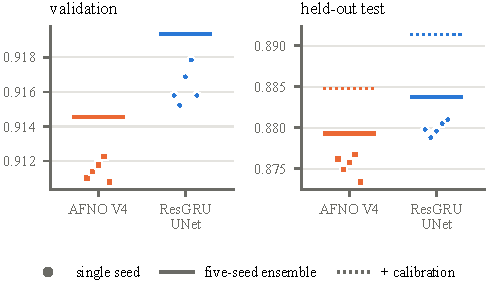
\includegraphics[width=\columnwidth]{fig_seed_spread.pdf}
\caption{Every seed of each finalist. The two families do not overlap on validation or on the held-out test.}
\label{fig:seeds}
\end{figure}

\textbf{Agreement of validation and test.} Fig.~\ref{fig:valtest} plots validation against test for the 25 network forecasts that have both: the five round-one networks, the other eight single seeds, the eight ensembles with and without calibration, and the four ablations. The Pearson correlation is 0.96 and the Spearman rank correlation 0.93; with persistence and ridge added, the Pearson correlation is 0.99 over 27 forecasts. Validation is optimistic in level (it chose each run's best epoch and fitted the calibration) but it orders the forecasts much as the test does, which is what the decision rules require. On the test inputs, the two five-seed ensembles make similar forecasts: their log forecasts correlate at 0.996 and differ by 0.079 on average, about 8\%.

\begin{figure}[!htb]
\centering
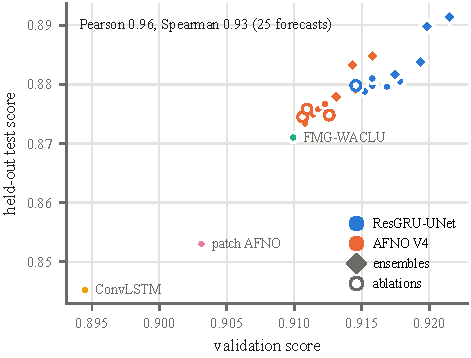
\includegraphics[width=\columnwidth]{fig_val_test.pdf}
\caption{Validation against held-out test for the 25 network forecasts that have both scores. Filled circles: single seeds; diamonds: ensembles, with and without calibration; open circles: single-change ablations.}
\label{fig:valtest}
\end{figure}

\subsection{Regression Metrics and Lead Time}
Table~\ref{tab:regression} gives MAE, RMSE, $R^2$ and skill on validation for every model. Every network beats all three baselines on every metric. The ResGRU-UNet ensemble has 31.8\% lower RMSE and 39.4\% lower MAE than persistence. Ridge improves on persistence on validation (score 0.8637) but barely on the test set (0.7951 against 0.7910). Appendix~\ref{app:regfull} adds every seed, every ensemble, the ablations and the same metrics in log space.

\begin{table}[!htb]
\centering
\caption{Validation regression metrics (MAE, RMSE in \ugm) over all $5.9\times10^7$ values, with the benchmark score $S$. Skill: lower RMSE than persistence. Calibration rows: factors fitted with one month left out. The hybrid row is out of fold}
\label{tab:regression}
\setlength{\tabcolsep}{2.6pt}
\begin{tabular}{@{}lrrrrr@{}}
\toprule
Model & MAE & RMSE & $R^2$ & Skill & $S$ \\
\midrule
Persistence & 10.44 & 26.46 & 0.767 & 0.0\% & 0.8515 \\
Seasonal naive (24 h) & 11.53 & 26.80 & 0.761 & $-1.3$\% & 0.7907 \\
Ridge regression & 8.51 & 21.48 & 0.847 & 18.8\% & 0.8637 \\
\midrule
\multicolumn{6}{@{}l}{\textit{Round one, seed 42}} \\
patch AFNO & 6.85 & 19.02 & 0.880 & 28.1\% & 0.9031 \\
ConvLSTM & 7.05 & 18.93 & 0.881 & 28.5\% & 0.8945 \\
FMG-WACLU & 7.14 & 19.32 & 0.876 & 27.0\% & 0.9099 \\
AFNO V4 & 7.31 & 20.17 & 0.865 & 23.8\% & 0.9110 \\
ResGRU-UNet & 6.57 & 18.57 & 0.885 & 29.8\% & 0.9158 \\
\midrule
\multicolumn{6}{@{}l}{\textit{Five-seed means}} \\
AFNO V4 & 6.99 & 19.45 & 0.874 & 26.5\% & 0.9145 \\
\ + calibration & 7.76 & 20.90 & 0.855 & 21.0\% & 0.9149 \\
ResGRU-UNet & \textbf{6.32} & 18.04 & 0.892 & 31.8\% & 0.9193 \\
\ + calibration & 7.12 & 19.71 & 0.871 & 25.5\% & \textbf{0.9210} \\
\ + LightGBM (hybrid) & 6.42 & \textbf{17.75} & \textbf{0.895} & \textbf{32.9\%} & 0.9051 \\
\bottomrule
\end{tabular}
\end{table}

\begin{figure*}[!tb]
\centering
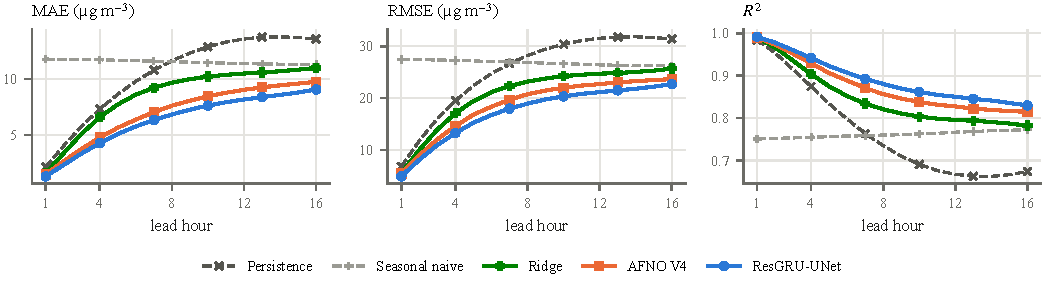
\includegraphics[width=\textwidth]{fig_lead_metrics.pdf}
\caption{Validation MAE, RMSE and $R^2$ by lead hour (five-seed means, no calibration). ResGRU-UNet is best at every hour. Seasonal naive overtakes persistence from hour 8, when the daily cycle outweighs the last observed state.}
\label{fig:lead}
\end{figure*}

Fig.~\ref{fig:lead} and Table~\ref{tab:lead} in Appendix~\ref{app:supp} show the error growing with lead time: ResGRU-UNet's $R^2$ falls from 0.992 at hour 1 to 0.830 at hour 16, and persistence's from 0.985 to 0.674. Seasonal naive is flat over the horizon and overtakes persistence on all three metrics from hour 8. Fig.~\ref{fig:terms} in Appendix~\ref{app:extra} splits the score into its three terms. ResGRU-UNet is better on all three at every hour; the score gap grows from $+0.0018$ at hour 1 to about $+0.006$ at hours 10 to 15. Of the five-seed gap, 56\% comes from global SMAPE, 23\% from episode SMAPE and 22\% from episode correlation.

\textbf{Episode cells.} Table~\ref{tab:episode} splits the errors between the 1.8\% of values that are episodes and the rest. On episode cells every network is far better than every baseline: the ResGRU-UNet ensemble has an episode MAE of 15.68 against 27.63 for persistence. Ridge, which beats persistence overall, is worse than persistence on episode cells (MAE 30.93, $R^2$ 0.589 against 0.640): a linear model shared by all cells pulls the forecast toward typical values. Calibration shows the trade-off of Section~\ref{sec:theory} directly. It lowers the episode MAE of the ResGRU-UNet ensemble by 6.6\% (15.68 to 14.65) and raises the MAE on the other cells by 13.6\% (6.15 to 6.98); for AFNO V4 the changes are $-2.9$\% and $+11.7$\%.

\begin{table}[!htb]
\centering
\caption{Validation errors on episode cells ($n=1{,}082{,}178$) and on all other cells ($n=58{,}358{,}462$); MAE, RMSE in \ugm. Calibration: one month left out}
\label{tab:episode}
\setlength{\tabcolsep}{2.4pt}
\begin{tabular}{@{}lrrrrrr@{}}
\toprule
 & \multicolumn{3}{c}{Episode cells} & \multicolumn{3}{c}{Other cells} \\
\cmidrule(lr){2-4}\cmidrule(l){5-7}
Model & MAE & RMSE & $R^2$ & MAE & RMSE & $R^2$ \\
\midrule
Persistence & 27.63 & 60.22 & 0.640 & 10.12 & 25.41 & 0.771 \\
Seasonal naive & 46.15 & 84.61 & 0.289 & 10.89 & 24.47 & 0.787 \\
Ridge & 30.93 & 64.35 & 0.589 & 8.09 & 19.83 & 0.860 \\
AFNO V4, 5 seeds & 16.32 & 42.70 & 0.819 & 6.81 & 18.75 & 0.875 \\
\ + calibration & 15.84 & 41.75 & 0.827 & 7.61 & 20.31 & 0.854 \\
ResGRU-UNet, 5 seeds & 15.68 & 40.23 & 0.839 & 6.15 & 17.37 & 0.893 \\
\ + calibration & 14.65 & 38.66 & 0.852 & 6.98 & 19.18 & 0.869 \\
\bottomrule
\end{tabular}
\end{table}

\subsection{Finding 3: Rankings and Post-Processing Depend on the Metric}
\label{sec:finding3}
ResGRU-UNet is first on all six measures in Fig.~\ref{fig:rank}, but the other four reorder. AFNO V4 is second on the benchmark score yet last on MAE, RMSE and $R^2$; ConvLSTM is last on the score yet second on RMSE and $R^2$. The score is relative and focused on episodes, while raw-scale MAE, RMSE and $R^2$ are dominated by high concentrations. A single metric would have given a misleading ranking of the weaker networks.

\begin{figure}[!htb]
\centering
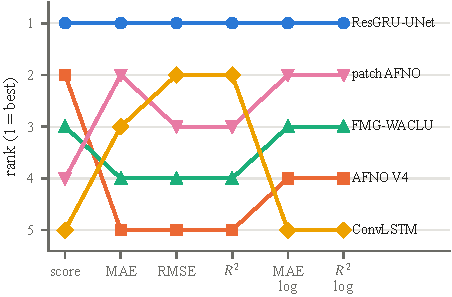
\includegraphics[width=\columnwidth]{fig_rank_by_metric.pdf}
\caption{Round-one ranks (seed 42) under six measures. Only ResGRU-UNet keeps its rank under every measure.}
\label{fig:rank}
\end{figure}

Calibration raises the score but worsens MAE, RMSE and $R^2$ for both finalists (Fig.~\ref{fig:calib}): the ResGRU-UNet ensemble moves from MAE 6.32 to 7.12 while its score rises from 0.9193 to 0.9210. The factors push forecasts up, which the episode terms reward and absolute and squared errors penalize. The uncalibrated mean is the better model for MAE, RMSE and $R^2$; the calibrated one is better for the benchmark score. The ML + DL hybrid of Section~\ref{sec:hybrid} shows the same trade-off in reverse.

\begin{figure}[!htb]
\centering
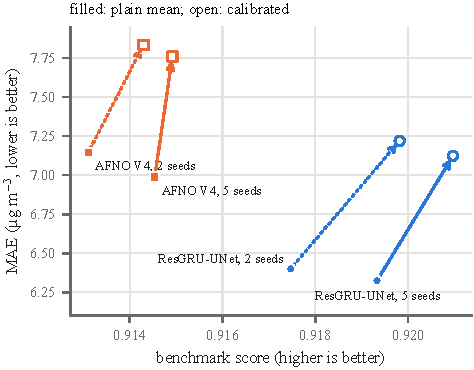
\includegraphics[width=\columnwidth]{fig_calibration.pdf}
\caption{Calibration moves both finalists to a higher score and a higher MAE (validation; in sample for 2 seeds, leave one month out for 5 seeds).}
\label{fig:calib}
\end{figure}

Fig.~\ref{fig:calibscales} in Appendix~\ref{app:supp} shows the fitted factors. They rise with lead time for both finalists and for every choice of fitting months, and they are larger for ResGRU-UNet (1.01 at hour 1 to 1.10 from hour 14) than for AFNO V4 (1.00 to 1.08). Leaving the scored month out costs little: 0.9210 against 0.9215 in sample for ResGRU-UNet and 0.9149 against 0.9158 for AFNO V4. The factors fitted without October are the largest, that is, October itself favours the smallest shift.

\FloatBarrier
\section{Analysis}
\label{sec:analysis}
\subsection{Where ResGRU-UNet Wins}
It is ahead in all four validation months (Table~\ref{tab:months} in Appendix~\ref{app:supp}), lower in SMAPE in five of six concentration bins and equal in the highest (Table~\ref{tab:bins} in Appendix~\ref{app:supp}), and lower in every decile of cells ranked by their mean concentration (Table~\ref{tab:deciles} in Appendix~\ref{app:extra}). Both models under-predict episode cells (mean log bias $-0.160$ for AFNO V4 and $-0.157$ for ResGRU-UNet) and over-predict the other cells ($+0.084$ and $+0.062$), most of all in the cleanest bin (Fig.~\ref{fig:where}, middle). ResGRU-UNet's smaller over-prediction outside episodes is consistent with its larger gain in the global term.

\begin{figure*}[!tb]
\centering
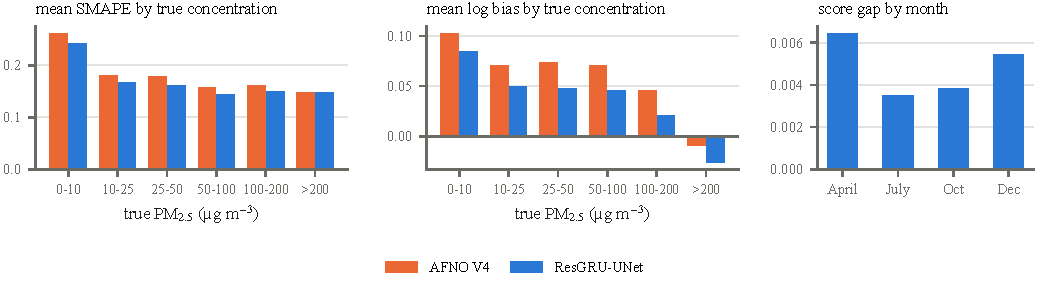
\includegraphics[width=\textwidth]{fig_where.pdf}
\caption{Five-seed means on validation. Left: mean SMAPE by true concentration. Middle: mean log bias (positive: too high). Right: score gap by month (ResGRU-UNet minus AFNO V4).}
\label{fig:where}
\end{figure*}

Fig.~\ref{fig:maps} maps the time-averaged errors. \PM{} and the errors of persistence concentrate over the Indo-Gangetic Plain and the eastern coal belt; ResGRU-UNet removes much of that error. It has lower MAE than AFNO V4 in 90.5\% of cells and lower SMAPE in 94.7\% (Fig.~\ref{fig:smape} in Appendix~\ref{app:extra}), with the largest gains over the Indo-Gangetic Plain and central India. The median per-cell $R^2$ over time is 0.872 for ResGRU-UNet, 0.846 for AFNO V4 and 0.694 for persistence; it is lowest north of 32$^\circ$N (median 0.764), where the air is cleanest (13.8 against 42.3~\ugm{} south of it). Fig.~\ref{fig:case} in the same appendix shows the window with the most episode cells.

\begin{figure*}[!tb]
\centering
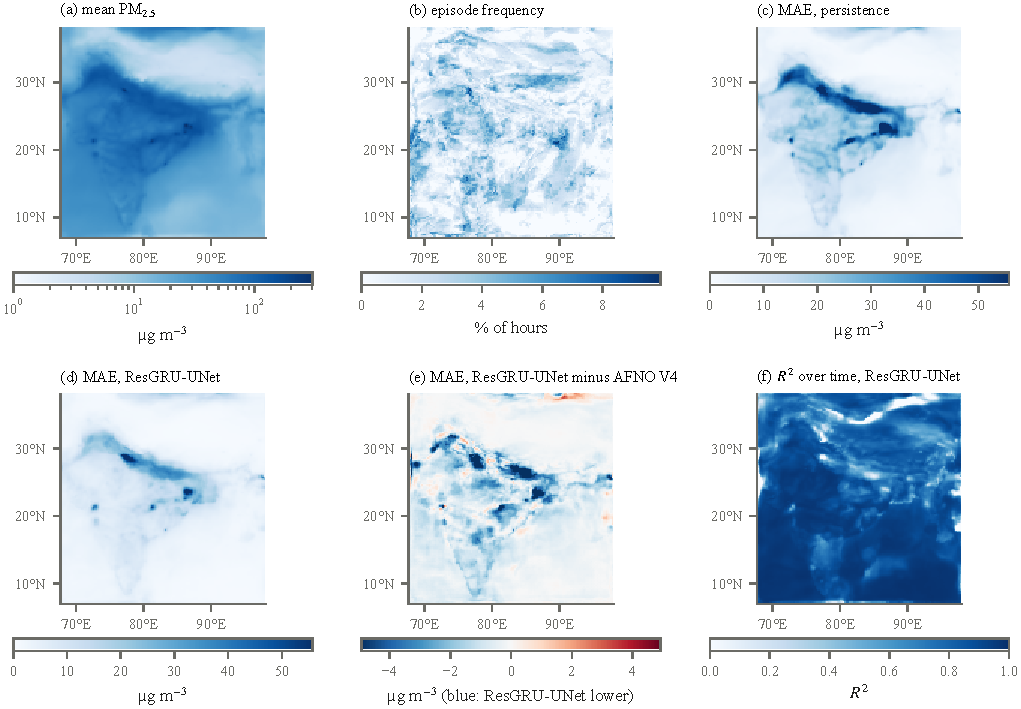
\includegraphics[width=\textwidth]{fig_maps.pdf}
\caption{Time-averaged validation maps. (a) Mean \PM. (b) Share of hours that are episodes. (c, d) MAE of persistence and of the ResGRU-UNet five-seed mean. (e) MAE difference, ResGRU-UNet minus AFNO V4. (f) $R^2$ of each cell's time series, ResGRU-UNet.}
\label{fig:maps}
\end{figure*}

\subsection{Why It Wins: Ablations and Training Curves}
\label{sec:ablation}
We tested four hypotheses, each with one change to one finalist and one seed (Table~\ref{tab:ablations}), with predictions written down first. A change counts only if it moves validation by more than $\max(2\,\mathrm{sd}, 0.002)$ from its family's five-seed mean, which is 0.002 for AFNO V4 and 0.00208 for ResGRU-UNet:
\begin{itemize}
\item H1: AFNO V4's skips keep only the last hour and the mean;
\item H2: the FFT wraps opposite edges of a non-periodic map;
\item H3: the soft threshold removes small details;
\item H4: ResGRU-UNet wins because of its recurrence over lead time.
\end{itemize}
None passes the threshold at one seed. H1 (skips that fuse all 10 hours, started equal to V4's fusion) moves AFNO V4 about a quarter of the way toward ResGRU-UNet. Replacing ResGRU-UNet's ConvGRU with per-lead convolution blocks of the same size costs about a third of the gap, yet it still beats every AFNO V4 seed: the recurrence is therefore not required for the win, although its contribution remains unresolved. Padding also strengthens the soft threshold, because the orthonormal FFT spreads the same energy over four times as many coefficients; H3 suggests this matters little.

\begin{table}[!htb]
\centering
\caption{Single-change ablations (seed 42). $d$: validation change from the family's five-seed mean; $d/G$: share of the 0.00484 gap. Threshold 0.002 (AFNO V4) and 0.00208 (ResGRU-UNet)}
\label{tab:ablations}
\setlength{\tabcolsep}{3pt}
\begin{tabular}{@{}lp{0.4\columnwidth}rrr@{}}
\toprule
 & Change & $d$ & $d/G$ & Test \\
\midrule
H1 & AFNO V4, skips fuse all 10 hours & $+0.00113$ & $+0.23$ & 0.8748 \\
H2 & AFNO V4, zero-padded FFT & $-0.00084$ & $-0.17$ & 0.8745 \\
H3 & AFNO V4, no soft threshold & $-0.00052$ & $-0.11$ & 0.8758 \\
H4 & ResGRU-UNet, ConvGRU replaced & $-0.00174$ & $-0.36$ & 0.8798 \\
\bottomrule
\end{tabular}
\end{table}

\textbf{A generalization gap.} The training curves (Fig.~\ref{fig:curves}; Table~\ref{tab:curves} in Appendix~\ref{app:supp}) show a pattern none of the AFNO changes altered. Every AFNO run reaches a lower training loss than ResGRU-UNet (0.053 to 0.054 against 0.064 to 0.068) but a higher validation loss: at a training loss of 0.09, its validation loss is 6.8\% higher on average. Its score peaks at epoch 4 or 5 and then falls by 0.009 to 0.010; ResGRU-UNet peaks at epoch 6 or 7 and falls by 0.003 to 0.005. Without its recurrence, ResGRU-UNet moves about 41\% of the way toward AFNO's validation loss. These observations are exploratory, but they suggest AFNO V4 fits the training months more and transfers less to new months. Its global, wrap-around spectral mixing, per-hour encoder and translator remain candidates for the cause.

\begin{figure}[!htb]
\centering
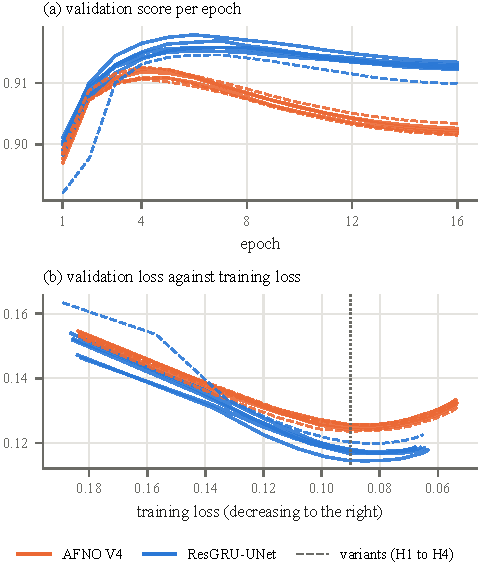
\includegraphics[width=\columnwidth]{fig_training_curves.pdf}
\caption{Training curves of the 12 ResGRU-UNet and AFNO V4 runs with per-epoch logs (AFNO V4 seeds 1 to 3, ResGRU-UNet seeds 42, 1337 and 1 to 3, and the four ablation variants): (a) validation score per epoch; (b) validation loss against training loss, with a dotted line at a training loss of 0.09.}
\label{fig:curves}
\end{figure}

\subsection{An ML + DL Hybrid}
\label{sec:hybrid}
We tested whether a classical model can correct the network. A LightGBM model \cite{ke2017lightgbm} predicts the error of the uncalibrated ResGRU-UNet five-seed ensemble in $\log(1+y)$, and the forecast is shifted by it. It uses 33 features per cell and lead hour: the 20 input channels at the last hour, $\log(1+y)$ at the nine earlier hours, the ensemble forecast, its change from the last hour, the spread of the five seeds, and the lead hour. One model serves all lead hours; it is fitted on every fourth cell in each direction (about 2.8 million rows per fold) with fixed settings: Huber loss ($\alpha=0.5$), 300 trees, learning rate 0.05, 31 leaves, at least 500 rows per leaf, row and feature subsampling 0.8, and L2 penalty 10. The rule was written before the run: fit on the validation windows of three months and predict the fourth, for all four months, and call the hybrid better only if its pooled score is higher and it wins in at least three months; only then would it be fitted on all four months and scored on the test set.

The hybrid did not improve the score. It scores lower in all four held-out months and 0.9051 against 0.9193 pooled (Table~\ref{tab:hybrid} and Fig.~\ref{fig:hybrid}). RMSE and $R^2$ improve slightly pooled (17.75 against 18.04; 0.895 against 0.892) and MAE is slightly worse (6.42 against 6.32), but episode SMAPE rises from 0.235 to 0.305. The regression gains are not uniform: RMSE falls in April and October and rises in July and December. This is the calibration trade-off in reverse, and it fits the theory of Section~\ref{sec:theory}: a symmetric loss in log space pulls forecasts toward the typical value, which removes the upward shift that the episode terms reward. The mean correction is 0.072 in log, about 7\%. The model relied most on the forecast's change from the last hour and on the seed spread (15\% and 13\% of its split gain), then on location, the ensemble forecast itself and the cell's climatology. The rule allowed a test submission only after a win. After the verdict, the hybrid was fitted on all four months and scored on the test set once, for the record: 0.8608, against 0.8838 for the uncalibrated ensemble it corrects (public part: 0.8775 against 0.8975). The test result agrees with the validation verdict.

\begin{table*}[!tb]
\centering
\caption{The hybrid, out of fold: fit on three validation months, predict the fourth. Ens.: uncalibrated ResGRU-UNet five-seed ensemble; Hyb.: ensemble + LightGBM correction. Windows: fitted/predicted. MAE, RMSE in \ugm}
\label{tab:hybrid}
\setlength{\tabcolsep}{4pt}
\begin{tabular}{@{}lccccccccccc@{}}
\toprule
 & & \multicolumn{2}{c}{Score $S$} & \multicolumn{2}{c}{Episode SMAPE} & \multicolumn{2}{c}{MAE} & \multicolumn{2}{c}{RMSE} & \multicolumn{2}{c}{$R^2$} \\
\cmidrule(lr){3-4}\cmidrule(lr){5-6}\cmidrule(lr){7-8}\cmidrule(lr){9-10}\cmidrule(l){11-12}
Held-out month & Windows & Ens. & Hyb. & Ens. & Hyb. & Ens. & Hyb. & Ens. & Hyb. & Ens. & Hyb. \\
\midrule
April & 162/52 & 0.9162 & 0.8999 & 0.253 & 0.329 & 4.03 & 3.85 & 12.53 & 11.76 & 0.661 & 0.701 \\
July & 160/54 & 0.9091 & 0.8940 & 0.283 & 0.357 & 3.06 & 3.07 & 10.43 & 10.91 & 0.824 & 0.808 \\
October & 160/54 & 0.9271 & 0.9203 & 0.184 & 0.225 & 6.84 & 6.16 & 16.38 & 13.85 & 0.849 & 0.892 \\
December & 160/54 & 0.9249 & 0.9061 & 0.221 & 0.310 & 11.28 & 12.52 & 27.60 & 28.38 & 0.897 & 0.891 \\
\midrule
Pooled & 214 & 0.9193 & 0.9051 & 0.235 & 0.305 & 6.32 & 6.42 & 18.04 & 17.75 & 0.892 & 0.895 \\
\bottomrule
\end{tabular}
\end{table*}

\begin{figure*}[!tb]
\centering
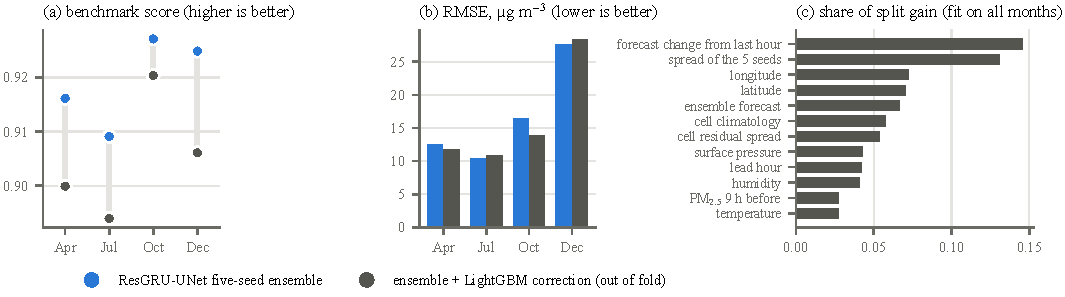
\includegraphics[width=\textwidth]{fig_hybrid.pdf}
\caption{The ML + DL hybrid. (a) Score in each held-out month: the correction lowers it every time. (b) RMSE in each held-out month: lower in April and October, higher in July and December. (c) The twelve features with the largest share of LightGBM's split gain, from a fit on all four months.}
\label{fig:hybrid}
\end{figure*}

\subsection{What the Linear Model Learned}
\label{sec:ridge}
The ridge baseline is the classical reference, and its weights show what a linear forecaster takes from the same inputs. The penalty hardly matters up to $10^2$ (Table~\ref{tab:ridgegrid} in Appendix~\ref{app:supp}); the chosen $\lambda=10^{-2}$ scores 0.8637 and zero weights give persistence's 0.8515 exactly, as they must. The inputs are standardized per cell, so the weights are comparable (Fig.~\ref{fig:ridge}). The weight on the last hour's \PM{} goes from $+0.09$ at hour 1 to $-1.72$ at hour 13, so the forecast relaxes from the last value as the lead grows. The diurnal anomaly (up to $+0.82$), \PM{} one hour earlier ($-0.19$ to $+0.57$), \PM{} nine and eight hours earlier (up to $+0.39$ and down to $-0.20$) and the tendency (up to $+0.13$) take the next largest weights; the other 23 weights stay within $\pm0.11$. The inputs are correlated, so single weights should not be read as causal effects. The linear model gains on persistence overall but loses on episode cells (Table~\ref{tab:episode}), and on the test set it barely improves on persistence; the gap from ridge (0.8637) to the networks (0.8945 to 0.9158) measures what nonlinear spatial modelling adds within the same pipeline.

\begin{figure}[!htb]
\centering
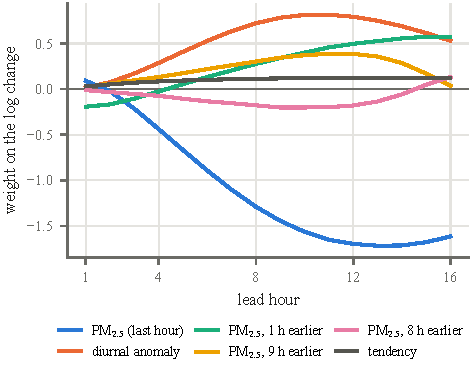
\includegraphics[width=\columnwidth]{fig_ridge_weights.pdf}
\caption{Ridge weights on the predicted log change by lead hour, for the six inputs with the largest weights (inputs standardized per cell). The other 23 weights stay within $\pm0.11$.}
\label{fig:ridge}
\end{figure}

\subsection{Cost}
\label{sec:cost}
ResGRU-UNet is also cheaper (Table~\ref{tab:cost}): 25.8 against 48.6~ms per window at inference, 0.23 against 1.36~GB of peak inference memory at batch 4, and about 190 against 338~s per training epoch on a T4. Parameter count does not predict cost or accuracy here. ConvLSTM has the most parameters, almost all in two spectral blocks, yet it is the fastest to train after patch AFNO and the weakest on the score; FMG-WACLU has the fewest and is the slowest, probably because it runs three ConvLSTMs at full resolution.

\begin{table}[!htb]
\centering
\caption{Cost on one NVIDIA T4. Training: seconds per epoch and minutes per run (mean over the round-one and seed runs). Inference was timed for the finalists only}
\label{tab:cost}
\setlength{\tabcolsep}{3pt}
\begin{tabular}{@{}lrrrrr@{}}
\toprule
Network & Params & s/epoch & min/run & ms/window & GB \\
\midrule
ResGRU-UNet & 7.12M & 190 & 51 & 25.8 & 0.23 \\
AFNO V4 & 6.98M & 338 & 90 & 48.6 & 1.36 \\
FMG-WACLU & 3.45M & 530 & 141 & & \\
patch AFNO & 5.71M & 56 & 15 & & \\
ConvLSTM & 19.0M & 69 & 19 & & \\
\bottomrule
\end{tabular}
\end{table}

\FloatBarrier
\section{Discussion}
\label{sec:discussion}
\subsection{Why the Pipeline Dominates}
The pipeline determines the starting point of every network. With the persistence residual and a zero-initialized head, an untrained network already scores 0.8515 on validation, and the best single network adds 0.064 to that. The pipeline changes act on every network at once: a validation split that measures what the test measures, inputs that carry the transport and mixing physics, a loss that matches the score, and post-processing that the score rewards. The network then determines how much of the remaining error is learned. With 2{,}257 training windows from four months, the data limit how much any architecture can show; Table~\ref{tab:v4steps} shows that even the smallest pipeline step, a two-seed ensemble, moved the test score about as much as the choice between the two best networks at one seed. The practical consequence is that networks should be compared only after the pipeline has been fixed.

\subsection{Local Mixing Suits This Problem}
In 16 hours, \PM{} moves about 10 to 12 cells at the mean and RMS winds (Appendix~\ref{app:cost}). A convolutional encoder with a recurrent core covers that radius; ResGRU-UNet's encoder alone reaches about 14 cells. AFNO mixes the whole map in every block and treats opposite edges as neighbours, which a non-periodic map of India does not need. The training curves show AFNO V4 fitting the training months more and doing worse on new months, and none of the three AFNO changes we tested closed the gap. These observations are consistent with a local inductive bias suiting a local transport problem, but they do not prove it: the ablations used one seed, and the candidate causes (global mixing, the per-hour encoder, the translator) were not all tested.

\subsection{Conditions That May Favour an Operator}
We did not test conditions that could favour a global operator, and we list them as open questions rather than findings: longer horizons, where transport exceeds a convolutional receptive field; global or periodic domains, where the FFT's wrap-around is correct; and much larger training sets, where a weaker inductive bias costs less. Each of these is a direct extension of the present design, with the pipeline held fixed.

\subsection{Choosing the Metric}
The benchmark score and the regression metrics disagree about the weaker networks and about calibration. This is expected when a point forecast is scored by different functions \cite{gneiting2011}: the episode terms reward an upward shift that absolute and squared errors penalize. The forecast should therefore be chosen for its use. A user who needs concentrations with small absolute error should take the uncalibrated ensemble; a user scored on episode detection, as the benchmark is, should take the calibrated one. For this reason we report both.

\subsection{Recommendations}
For controlled comparisons of spatio-temporal forecasters we suggest:
\begin{itemize}
\item fix the whole pipeline (inputs, split, loss, recipe, post-processing) and change only the network;
\item validate on a temporal hold-out with a gap at least one window long, and check that validation orders forecasts as an untouched test does;
\item write the decision rule before each stage, run several seeds, and compare seeds pairwise and with a block bootstrap;
\item report several metrics, including the raw-scale ones, and say which forecast is best for which;
\item start every network at persistence with a residual output, so training only learns the departure from it.
\end{itemize}

\section{Threats to Validity}
\label{sec:threats}
\textbf{External validity.} The data are simulations, not measurements, and skill on WRF-Chem fields need not carry over to monitored \PM. Training covers one month per season of one year, and the test set comes from the following year on the same grid.

\textbf{Internal validity.} The recipe was tuned for AFNO V4, which if anything favours it; ResGRU-UNet was not tuned. The later rounds were designed after round one's result. The pipeline gain bundles several changes that we did not separate for the three networks of Table~\ref{tab:samepipe}, and patch AFNO's gain includes its bug fix.

\textbf{Construct validity.} The score's weights are not disclosed; we assume equal weights on validation. The score is a composite of relative error and correlation focused on episodes, so it does not measure raw-scale accuracy, which is why we also report MAE, RMSE and $R^2$.

\textbf{Statistical conclusion validity.} There is one validation period and one test set. Validation picked each run's best epoch and fitted the calibration, so validation scores are optimistic; the test set is the only untouched measure, and it reports only the benchmark score. Adjacent bootstrap blocks overlap in time, and the ablations use one seed each. The hybrid was tested in one fixed configuration, on the validation windows that also chose each network's best epoch; its test score was taken after the verdict and did not inform it.

\section{Conclusion}
\label{sec:conclusion}
For 16-hour \PM{} forecasting over India, the pipeline mattered more than the network. Physics channels for mixing and transport, a log-space persistence residual, validation that reproduces the test, a loss matched to the score, and ensembling with calibration gave the same network a gain 6 to 8 times the gap between the two best networks. Inside one fixed pipeline, a plain convolutional-recurrent U-Net beat the Fourier neural operator hybrid on every seed pair, both parts of the test set, every lead hour, month and regression metric, and it is also cheaper to run. No single component we tested explains the gap; the Fourier model generalizes less well across months, which fits a transport problem that is local and not periodic. A gradient-boosted correction of the ensemble lowered squared error but not the benchmark score.

Four extensions remain open: separating the pipeline gain into its parts for each network; testing the same comparison on monitored \PM{} and at longer horizons; repeating the ablations with several seeds; and training a hybrid correction on the score's own terms, as the networks are.

\section*{Reproducibility}
The code is at \url{https://github.com/Vetri-78640/pm2.5-backbone-study-pipeline-over-backbone}: the shared pipeline and every network (\texttt{src/}), the notebook builders and Kaggle tools (\texttt{scripts/}), the dry runs, port check and config test (\texttt{tests/}), six local notebooks with outputs (\texttt{notebooks/}; \texttt{notebooks/kaggle/} holds the Kaggle notebooks exactly as they ran, with their run logs), the study settings (\texttt{configs/}), the run records (\texttt{results/}), the AFNO V4 script and the original notebooks of the ported networks (\texttt{reference/}), and this paper with its figures (\texttt{paper/}). Every table and figure in this paper is built from the files in \texttt{results/}. The data are not included; see \texttt{data/README.md}. The five ResGRU-UNet networks, with their calibration factors and normalization statistics, are at \url{https://www.kaggle.com/models/imvetri0/resgru-unet-pm25}.

\FloatBarrier
\begin{thebibliography}{99}
\bibitem{pandey2021} A. Pandey \emph{et al.}, ``Health and economic impact of air pollution in the states of India: The Global Burden of Disease Study 2019,'' \emph{Lancet Planet. Health}, vol. 5, no. 1, pp. e25--e38, 2021.
\bibitem{grell2005} G. A. Grell, S. E. Peckham, R. Schmitz, S. A. McKeen, G. Frost, W. C. Skamarock, and B. Eder, ``Fully coupled `online' chemistry within the WRF model,'' \emph{Atmos. Environ.}, vol. 39, no. 37, pp. 6957--6975, 2005.
\bibitem{li2021fno} Z. Li, N. Kovachki, K. Azizzadenesheli, B. Liu, K. Bhattacharya, A. Stuart, and A. Anandkumar, ``Fourier neural operator for parametric partial differential equations,'' in \emph{Proc. ICLR}, 2021.
\bibitem{guibas2022afno} J. Guibas, M. Mardani, Z. Li, A. Tao, A. Anandkumar, and B. Catanzaro, ``Efficient token mixing for transformers via adaptive Fourier neural operators,'' in \emph{Proc. ICLR}, 2022.
\bibitem{shi2015convlstm} X. Shi, Z. Chen, H. Wang, D.-Y. Yeung, W.-k. Wong, and W.-c. Woo, ``Convolutional LSTM network: A machine learning approach for precipitation nowcasting,'' in \emph{Proc. NeurIPS}, 2015, pp. 802--810.
\bibitem{ballas2016convgru} N. Ballas, L. Yao, C. Pal, and A. Courville, ``Delving deeper into convolutional networks for learning video representations,'' in \emph{Proc. ICLR}, 2016.
\bibitem{wightman2021} R. Wightman, H. Touvron, and H. J\'{e}gou, ``ResNet strikes back: An improved training procedure in timm,'' arXiv:2110.00476, 2021.
\bibitem{bello2021} I. Bello, W. Fedus, X. Du, E. D. Cubuk, A. Srinivas, T.-Y. Lin, J. Shlens, and B. Zoph, ``Revisiting ResNets: Improved training and scaling strategies,'' in \emph{Adv. Neural Inf. Process. Syst.}, vol. 34, 2021.
\bibitem{liu2022convnext} Z. Liu, H. Mao, C.-Y. Wu, C. Feichtenhofer, T. Darrell, and S. Xie, ``A ConvNet for the 2020s,'' in \emph{Proc. IEEE/CVF Conf. Comput. Vis. Pattern Recognit. (CVPR)}, 2022, pp. 11976--11986.
\bibitem{zeng2023} A. Zeng, M. Chen, L. Zhang, and Q. Xu, ``Are transformers effective for time series forecasting?'' in \emph{Proc. AAAI Conf. Artif. Intell.}, vol. 37, no. 9, 2023, pp. 11121--11128.
\bibitem{kushwaha2025} A. Kushwaha and K. Gopalan, ``A comparison of lightweight deep learning models for particulate-matter nowcasting in the Indian subcontinent \& surrounding regions,'' arXiv:2511.11185, 2025.
\bibitem{bedi2025conoair} S. Bedi, K. Tiwari, Prathosh A. P., S. H. Kota, N. M. A. Krishnan \emph{et al.}, ``CoNOAir: A neural operator for forecasting carbon monoxide evolution in cities,'' arXiv:2501.06007, 2025.
\bibitem{pathak2022fourcastnet} J. Pathak \emph{et al.}, ``FourCastNet: A global data-driven high-resolution weather model using adaptive Fourier neural operators,'' arXiv:2202.11214, 2022.
\bibitem{dang2025adaptfno} H. V. Dang, B. D. G. Nguyen, P. C. H. Nguyen, and T.-S. Hy, ``AdaptFNO: Adaptive Fourier neural operator with dynamic spectral modes and multiscale learning for climate modeling,'' in \emph{NeurIPS Workshop on Machine Learning and the Physical Sciences}, 2025.
\bibitem{shi2017trajgru} X. Shi, Z. Gao, L. Lausen, H. Wang, D.-Y. Yeung, W.-k. Wong, and W.-c. Woo, ``Deep learning for precipitation nowcasting: A benchmark and a new model,'' in \emph{Proc. NeurIPS}, 2017.
\bibitem{ronneberger2015unet} O. Ronneberger, P. Fischer, and T. Brox, ``U-Net: Convolutional networks for biomedical image segmentation,'' in \emph{Proc. MICCAI}, 2015, pp. 234--241.
\bibitem{he2016} K. He, X. Zhang, S. Ren, and J. Sun, ``Deep residual learning for image recognition,'' in \emph{Proc. CVPR}, 2016, pp. 770--778.
\bibitem{gao2022simvp} Z. Gao, C. Tan, L. Wu, and S. Z. Li, ``SimVP: Simpler yet better video prediction,'' in \emph{Proc. CVPR}, 2022, pp. 3170--3180.
\bibitem{leinonen2021} J. Leinonen, ``Spatiotemporal weather data predictions with shortcut recurrent-convolutional networks: A solution for the Weather4cast challenge,'' arXiv:2111.02121, 2021.
\bibitem{melis2018} G. Melis, C. Dyer, and P. Blunsom, ``On the state of the art of evaluation in neural language models,'' in \emph{Proc. ICLR}, 2018.
\bibitem{lucic2018} M. Lucic, K. Kurach, M. Michalski, S. Gelly, and O. Bousquet, ``Are GANs created equal? A large-scale study,'' in \emph{Adv. Neural Inf. Process. Syst.}, vol. 31, 2018, pp. 700--709.
\bibitem{gneiting2011} T. Gneiting, ``Making and evaluating point forecasts,'' \emph{J. Amer. Statist. Assoc.}, vol. 106, no. 494, pp. 746--762, 2011.
\bibitem{goodwin1999} P. Goodwin and R. Lawton, ``On the asymmetry of the symmetric MAPE,'' \emph{Int. J. Forecast.}, vol. 15, no. 4, pp. 405--408, 1999.
\bibitem{roberts2017} D. R. Roberts \emph{et al.}, ``Cross-validation strategies for data with temporal, spatial, hierarchical, or phylogenetic structure,'' \emph{Ecography}, vol. 40, no. 8, pp. 913--929, 2017.
\bibitem{kaufman2012} S. Kaufman, S. Rosset, C. Perlich, and O. Stitelman, ``Leakage in data mining: Formulation, detection, and avoidance,'' \emph{ACM Trans. Knowl. Discov. Data}, vol. 6, no. 4, Art. no. 15, 2012.
\bibitem{kunsch1989} H. R. K\"{u}nsch, ``The jackknife and the bootstrap for general stationary observations,'' \emph{Ann. Statist.}, vol. 17, no. 3, pp. 1217--1241, 1989.
\bibitem{bouthillier2021} X. Bouthillier \emph{et al.}, ``Accounting for variance in machine learning benchmarks,'' in \emph{Proc. Mach. Learn. Syst. (MLSys)}, vol. 3, 2021.
\bibitem{hyndman2021} R. J. Hyndman and G. Athanasopoulos, \emph{Forecasting: Principles and Practice}, 3rd ed. Melbourne, Australia: OTexts, 2021.
\bibitem{hoerl1970} A. E. Hoerl and R. W. Kennard, ``Ridge regression: Biased estimation for nonorthogonal problems,'' \emph{Technometrics}, vol. 12, no. 1, pp. 55--67, 1970.
\bibitem{loshchilov2019} I. Loshchilov and F. Hutter, ``Decoupled weight decay regularization,'' in \emph{Proc. ICLR}, 2019.
\bibitem{smith2019} L. N. Smith and N. Topin, ``Super-convergence: Very fast training of neural networks using large learning rates,'' in \emph{Proc. SPIE}, vol. 11006, 2019.
\bibitem{wu2018} Y. Wu and K. He, ``Group normalization,'' in \emph{Proc. ECCV}, 2018, pp. 3--19.
\bibitem{polyak1992} B. T. Polyak and A. B. Juditsky, ``Acceleration of stochastic approximation by averaging,'' \emph{SIAM J. Control Optim.}, vol. 30, no. 4, pp. 838--855, 1992.
\bibitem{lakshminarayanan2017} B. Lakshminarayanan, A. Pritzel, and C. Blundell, ``Simple and scalable predictive uncertainty estimation using deep ensembles,'' in \emph{Proc. NeurIPS}, 2017, pp. 6402--6413.
\bibitem{ke2017lightgbm} G. Ke \emph{et al.}, ``LightGBM: A highly efficient gradient boosting decision tree,'' in \emph{Adv. Neural Inf. Process. Syst.}, vol. 30, 2017, pp. 3146--3154.
\bibitem{aisehack2026} ANRF AISEHack 2026, Phase 2, Theme 2: pollution forecasting (IIT Delhi), Kaggle, 2026. [Online]. Available: \url{https://www.kaggle.com/competitions/anrf-aise-hack-phase-2-theme-2-pollution-forecasting-iitd}
\bibitem{cleveland1990} R. B. Cleveland, W. S. Cleveland, J. E. McRae, and I. Terpenning, ``STL: A seasonal-trend decomposition procedure based on loess,'' \emph{J. Off. Stat.}, vol. 6, no. 1, pp. 3--73, 1990.
\bibitem{iyer2013} U. S. Iyer and P. E. Raj, ``Ventilation coefficient trends in the recent decades over four major Indian metropolitan cities,'' \emph{J. Earth Syst. Sci.}, vol. 122, no. 2, pp. 537--549, 2013.
\bibitem{staniforth1991} A. Staniforth and J. C\^{o}t\'{e}, ``Semi-Lagrangian integration schemes for atmospheric models: A review,'' \emph{Mon. Weather Rev.}, vol. 119, no. 9, pp. 2206--2223, 1991.
\bibitem{koenker1978} R. Koenker and G. Bassett Jr., ``Regression quantiles,'' \emph{Econometrica}, vol. 46, no. 1, pp. 33--50, 1978.
\end{thebibliography}

\onecolumn
\appendices
\raggedbottom

\section{Data Exploration}
\label{app:eda}
Table~\ref{tab:monthstats} summarizes \PM{} in each training month and in the test inputs. The distribution is right-skewed in every month (skewness 5.1 on the raw scale and 0.13 after the log), and December has both the highest mean and the largest gap between mean and median. The highest monthly mean cell lies at 23.54$^\circ$N, 86.42$^\circ$E in April, July and October (177, 170 and 327~\ugm) and at 28.56$^\circ$N, 77.30$^\circ$E in December (466~\ugm).

\begin{table}[!htbp]
\centering
\caption{\PM{} by month (\ugm, all cells and hours)}
\label{tab:monthstats}
\begin{tabular}{@{}lrrrr@{}}
\toprule
Month & Mean & Median & 99th pct. & Max \\
\midrule
April 2016 & 22.4 & 16.2 & 119 & 2534 \\
July 2016 & 15.4 & 10.1 & 79 & 843 \\
October 2016 & 37.2 & 24.7 & 183 & 2850 \\
December 2016 & 59.1 & 23.7 & 366 & 1538 \\
Test inputs (2017) & 34.5 & 16.9 & 232 & 1519 \\
\bottomrule
\end{tabular}
\end{table}

The memory of the field fades over the horizon. The autocorrelation of $\log(1+y)$ is 0.978 at a lag of one hour, 0.728 at 6 hours, 0.535 at 12 hours and 0.571 at 24 hours, where the daily cycle brings it back up. The standard deviation of its change grows from 0.101 after one hour to 0.286, 0.419, 0.485 and 0.505 after 4, 8, 12 and 16 hours. The mean 10-m wind is 4.24~m/s and its RMS 4.97~m/s, so \PM{} travels 244 to 286~km in 16 hours, or 9.8 to 11.5 cells. In the April files, the emission fields are nonzero in 4\% (biomass-burning NMVOC) to 98\% of cell-hours, with maxima from $8\times10^{-9}$ to $7\times10^{-6}$; at that scale and without stated units they were left out.

\section{Development History}
\label{sec:history}
The pipeline of Sections~\ref{sec:method} and~\ref{sec:setup} was not designed at once. It grew over seven iterations, each started by a problem that the previous one exposed; the controlled study is iteration 8. Table~\ref{tab:iterations} lists each move and its reason, and Fig.~\ref{fig:evolution} shows the test score. Iterations 1 to 4 were chosen on a random validation split, which leaked (Section~\ref{sec:setup}), and on feedback from the public part of the test set, so only their test scores are comparable.

\begin{table}[!htbp]
\centering
\caption{Development iterations: what changed, why, and the held-out test score}
\label{tab:iterations}
\begin{tabular}{@{}c>{\raggedright\arraybackslash}p{0.39\textwidth}>{\raggedright\arraybackslash}p{0.41\textwidth}r@{}}
\toprule
\# & Change & Why & Test \\
\midrule
1 & AFNO on $4\times4$ patches, random split & first model: spectral mixing as in global weather models \cite{pathak2022fourcastnet} & 0.8218 \\
2 & U-Net + ConvGRU; output added to the last hour; log Huber loss & AFNO stalled below 0.83; keep local detail and sharp peaks & 0.8506 \\
3 & fine-tunes: 20 times the loss on missed episode peaks, then pinball loss ($q=0.75$) & peaks were under-predicted & 0.8594 \\
4 & blends with models trained at $q=0.85$ and $0.90$ & a stronger upward shift & 0.8648 \\
5 & temporal hold-out; AFNO with a SimVP translator, blended with ResGRU-UNet & the random split leaked & 0.8561 \\
6 & V3: official STL episodes, exact score for selection, 12-h gap, hour estimation & validation must measure what the test measures & 0.8609 \\
7 & V4: physics channels, multiscale block, lead-hour weights, 2 seeds, calibration & V3's diagnosis: long-lead errors and a global-episode trade-off & 0.8833 \\
8 & ResGRU-UNet in the V4 pipeline, 5 seeds, calibration & compare networks with the pipeline fixed & \textbf{0.8914} \\
\bottomrule
\end{tabular}
\end{table}

\begin{figure}[!htbp]
\centering
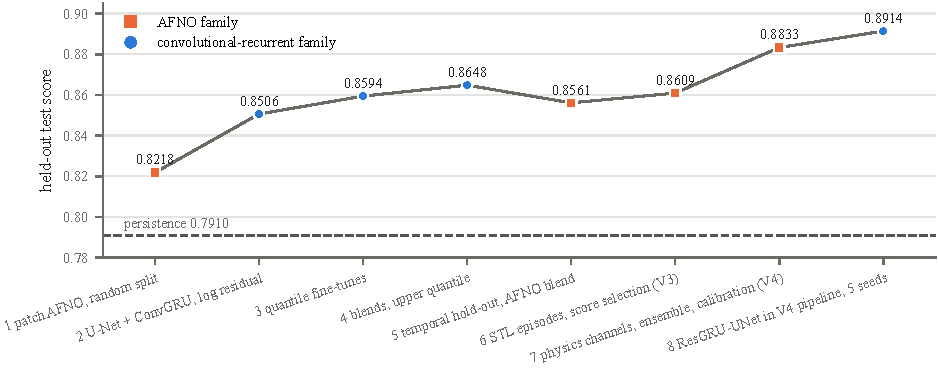
\includegraphics[width=\textwidth]{fig_pipeline_evolution.pdf}
\caption{Held-out test score at each development iteration. The dashed line is persistence (0.7910). Iteration 5 rebuilt the pipeline on a leak-free split and scored below iteration 4; the rebuilt pipeline overtakes it from iteration 6.}
\label{fig:evolution}
\end{figure}

\textbf{1 to 2: from patch AFNO to ResGRU-UNet.} The first models followed FourCastNet: AFNO on $4\times4$ patches, trained on a random split. They stalled below 0.83 on the test set. We attributed this to the global spectral layers acting as low-pass filters that blurred sharp spikes, and moved to a U-Net with full-resolution skips for local detail, a ConvGRU, and an output added to the last observed hour. The score rose to 0.8506. Later checks showed that this explanation was wrong. The patch model's spectral step applied the same complex matrix at every frequency, so apart from its soft threshold it was almost linear and local; a bug also discarded the imaginary half of every filtered spectrum; and each $4\times4$ patch was rebuilt by one linear layer with no skips. Three things had changed at once (the persistence residual, the skips and a log-space loss), and persistence alone is already strong.

\textbf{2 to 4: shifting forecasts up.} The base ResGRU-UNet under-predicted peaks. We attributed this to losses that pull forecasts toward the centre and fine-tuned it in steps: a loss 20 times larger on under-predicted episode cells, then a pinball loss at the 0.75 quantile \cite{koenker1978}, then blends with models trained at the 0.85 and 0.90 quantiles. The test score rose at every step, from 0.8506 to 0.8648. This explanation was wrong, since SMAPE is symmetric in the log ratio (Section~\ref{sec:theory}), but the change helped for a different reason: episode cells are picked where the truth turned out high, so upward-shifted forecasts score better on the episode terms. Scaling forecasts by hand did not help. ``Physics multipliers'' that raised stagnant cells by 25\% and all other cells by 12\% lost 0.006, because the 98\% of background cells pay for the shift, and a geometric blend with an AFNO member lost 0.008. Grafting four physics channels onto trained weights failed with NaN values.

\textbf{4 to 5: a leak-free split.} The random split gave an episode correlation near 0.98 for models that scored about 0.86 on the test set: with overlapping windows, it puts near-copies of every validation window into training. Iteration 5 held out the last 15 to 20\% of each month and rebuilt the model as AFNO with a SimVP-style temporal translator \cite{gao2022simvp}. Its best test score, 0.8561, came from a blend with ResGRU-UNet and was below iteration 4. The leak-free split did not raise the score, but it made model selection reliable. Selection still used the wrong target, however: a proxy episode mask that marked 0.30\% of validation cells against about 2\% for the official one, checkpoints chosen on the validation loss, and no gap between training and validation windows.

\textbf{5 to 6: validation equal to the metric (V3).} V3 rewrote the pipeline so that validation measures exactly what the test measures: the official robust STL episodes, the exact score for choosing checkpoints, a 12-hour gap, per-cell normalization, a lead-hour embedding and weight averaging. It also fixed a hidden mismatch: the ResGRU-UNet models had been trained with the true hour of day but given hours 0 to 9 for every test window. In V3, training keeps the true hour, while validation and test windows get the estimated hour of Section~\ref{sec:physics}, so validation sees the same hour noise as the test. As one model with no blend, V3 reached 0.8609. Its validation also revealed a trade-off that the earlier pipelines could not show: global SMAPE kept improving after epoch 4 while episode SMAPE got worse.

\textbf{6 to 7: physics and calibration (V4).} V4 kept V3's pipeline and addressed that diagnosis with the ventilation, advection, tendency and diurnal-anomaly channels of Section~\ref{sec:physics}, one AFNO block at $35\times31$ for a middle scale \cite{dang2025adaptfno}, lead-hour weights because errors grow with lead time, two seeds, and per-hour calibration fitted on the leak-free hold-out. Calibration replaced the manual shifts of iterations 3 and 4 with one fitted step, and the physics channels, which had failed when grafted onto trained weights, worked when the network was trained with them from the start. The test score rose by 0.0224 to 0.8833 (Table~\ref{tab:v4steps} splits the gain).

\textbf{7 to 8: one pipeline for every network.} V4 was the best model, but its pipeline had changed together with its network: split, masks, inputs, loss, hour handling and post-processing. The other networks had been trained in older, leakier pipelines, so their scores could not be compared with V4's. We therefore moved every network into V4's pipeline. Each was ported unchanged except for its input width (20 channels); ConvLSTM and patch AFNO also received the residual output with a zero-initialized last layer, ConvLSTM lost its season input, and patch AFNO got its bug fix. Each port was checked against its original (Section~\ref{sec:arch}). Each round-one notebook first re-evaluated the original AFNO V4 checkpoint on its own validation set and would have stopped unless it reproduced the logged 0.9110; it did, to five decimals. The windows, masks, loss, recipe and seed are then the same for every network, so the network is the only difference. Table~\ref{tab:samepipe} shows what the pipeline alone did for the three networks whose original runs are known: each gained 0.025 to 0.031 on the test set.

\section{Architecture and Training Details}
\label{app:arch}\label{app:runs}\label{app:cost}
\subsection{Layers}
Table~\ref{tab:archdetail} lists the layers of the five networks as they ran in the study. All five end in the persistence residual: the predicted change is added to $\log(1+y_t)$, and the last layer starts at zero. ConvBlock denotes two $3\times3$ convolutions with GroupNorm and GELU, channel dropout between them, and a residual connection; the same block is used in AFNO V4, ResGRU-UNet and FMG-WACLU.

\begin{table}[!htbp]
\centering
\caption{Layers of the five networks (study versions)}
\label{tab:archdetail}
\setlength{\tabcolsep}{3pt}
\begin{tabular}{@{}>{\raggedright\arraybackslash}p{0.10\textwidth}>{\raggedright\arraybackslash}p{0.17\textwidth}>{\raggedright\arraybackslash}p{0.21\textwidth}>{\raggedright\arraybackslash}p{0.24\textwidth}>{\raggedright\arraybackslash}p{0.22\textwidth}@{}}
\toprule
Network & Input & Encoder & Mixing and temporal core & Decoder and output \\
\midrule
ResGRU-UNet & 10 hours $\times$ 20 channels stacked into 200 channels & ConvBlocks with 64, 128 and 256 channels at $140{\times}124$, $70{\times}62$ and $35{\times}31$; average pooling to $18{\times}16$; bottleneck ConvBlock (256) & ConvGRU ($3\times3$, 256 channels) unrolled for 16 steps with the bottleneck as constant input and initial state & per lead hour: $1\times1$ projection, three transposed-convolution steps with skips from all encoder levels (128, 64, 32 channels), $3\times3$ conv head \\
\addlinespace
AFNO V4 & each of the 10 hours separately (20 channels) & shared ConvBlocks with 64, 128 and 256 channels; one AFNO block at $35{\times}31$; six AFNO blocks at $18{\times}16$ (8 blocks of channels, MLP ratio 2, $\lambda=0.01$) & translator over time per cell: two 1-D inception layers (kernels 1, 3, 5, 7), a transposed convolution from 10 to 16 hours, two more inception layers; lead-hour embedding; two AFNO blocks per lead hour & U-Net decoder (128, 64, 32); each skip is a $1\times1$ fusion of the last hour and the mean over the 10 hours; $3\times3$ conv head \\
\addlinespace
FMG-WACLU & 20 channels per hour plus wind speed, direction ($\sin$, $\cos$) and divergence & conv embedding (32); ConvLSTM over the 10 hours (128); a second ConvLSTM rolls the inputs forward 16 hours, and a third encodes the forecast fields; a sigmoid gate mixes the two states & ConvBlocks (64, 128) and bottleneck (128); ConvGRU (128) over the 16 lead hours & per lead hour: decoder (64, 32, 16) with skips, $3\times3$ conv head \\
\addlinespace
ConvLSTM & 20 channels plus the \PM{} map shifted along the wind by bilinear sampling & ConvLSTM over the 10 hours at full resolution (32), BatchNorm; U-Net encoder (32, 64, 128) & bottleneck with 256 channels and two FNO spectral blocks keeping $8\times8$ modes (88\% of the parameters) & decoder (128, 64, 32); the head outputs all 16 hours at once \\
\addlinespace
patch AFNO & 10 hours stacked; $4\times4$ patch embedding to 256 dimensions; $35{\times}31$ tokens with a learned position embedding & none & eight spectral blocks (4 heads; one complex matrix per head shared by all frequencies; MLP ratio 4; dropout 0.1) & linear projection of each token to $16\times4\times4$ values, then unpatchify \\
\bottomrule
\end{tabular}
\end{table}

\subsection{Training Runs}
Table~\ref{tab:runs} lists the 15 training runs of the study. AFNO V4 seeds 42 and 1337 come from the V4 run and were re-evaluated, not retrained. Every run first reproduced the V4 checkpoint's validation score (Section~\ref{sec:verify}), and every run completed all 16 epochs on one NVIDIA T4 with PyTorch 2.11.

\begin{table}[!htbp]
\centering
\caption{The 15 training runs: parameters, best epoch, best validation score as logged during training (the analysis recomputation agrees within $10^{-5}$), seconds per epoch and minutes of training}
\label{tab:runs}
\setlength{\tabcolsep}{2.2pt}
\begin{tabular}{@{}llrrcccc@{}}
\toprule
Network & Stage & Seed & Params & Ep. & Val $S$ & s/ep & min \\
\midrule
ResGRU-UNet & round 1 & 42 & 7{,}122{,}113 & 7 & 0.91579 & 189 & 51 \\
FMG-WACLU & round 1 & 42 & 3{,}454{,}645 & 7 & 0.90992 & 530 & 141 \\
patch AFNO & round 1 & 42 & 5{,}708{,}800 & 9 & 0.90312 & 56 & 15 \\
ConvLSTM & round 1 & 42 & 19{,}001{,}840 & 7 & 0.89448 & 69 & 19 \\
ResGRU-UNet & round 2 & 1337 & 7{,}122{,}113 & 6 & 0.91523 & 186 & 50 \\
ResGRU-UNet & round 3 & 1 & 7{,}122{,}113 & 7 & 0.91687 & 191 & 51 \\
ResGRU-UNet & round 3 & 2 & 7{,}122{,}113 & 6 & 0.91784 & 190 & 51 \\
ResGRU-UNet & round 3 & 3 & 7{,}122{,}113 & 7 & 0.91578 & 190 & 51 \\
AFNO V4 & round 3 & 1 & 6{,}980{,}033 & 4 & 0.91178 & 338 & 90 \\
AFNO V4 & round 3 & 2 & 6{,}980{,}033 & 4 & 0.91227 & 338 & 90 \\
AFNO V4 & round 3 & 3 & 6{,}980{,}033 & 5 & 0.91080 & 338 & 90 \\
AFNO V4, H1 & ablation & 42 & 7{,}668{,}161 & 4 & 0.91259 & 344 & 92 \\
AFNO V4, H2 & ablation & 42 & 6{,}980{,}033 & 4 & 0.91062 & 559 & 149 \\
AFNO V4, H3 & ablation & 42 & 6{,}980{,}033 & 4 & 0.91094 & 346 & 92 \\
ResGRU-UNet, H4 & ablation & 42 & 7{,}126{,}977 & 7 & 0.91456 & 197 & 53 \\
\bottomrule
\end{tabular}
\end{table}

\subsection{Reach and Cost of the Operators}
\textbf{How far must a forecast see.} At the mean wind of 4.24~m/s, \PM{} travels 244~km in 16 hours: 9.8 cells, or 11.5 cells at the RMS wind. Table~\ref{tab:opcost} compares the reach and cost of the main operators for $N$ cells, $d$ channels and kernel size $k$. A $3\times3$ convolution reaches one more cell per layer: ResGRU-UNet's encoder alone reaches about 14 cells, and each ConvGRU step at $18\times16$ adds about 8 more, so it covers the needed radius. AFNO mixes the whole map in every block, at a cost close to linear in $N$, but transport over 16 hours does not need global reach.

\begin{table}[!htbp]
\centering
\caption{Cost and reach per layer ($N$ cells, $d$ channels, $b$ blocks, $N_f$ Fourier modes)}
\label{tab:opcost}
\setlength{\tabcolsep}{4pt}
\begin{tabular}{@{}lll@{}}
\toprule
Operator & Cost (multiply-adds) & Reach per layer \\
\midrule
Self-attention & $2N^2d$ & whole map \\
AFNO block & $\approx 2.5\,dN\log_2N + 8N_fd^2/b$ & whole map \\
Convolution $k\times k$ & $Nk^2d_{\text{in}}d_{\text{out}}$ & $+(k-1)/2$ cells \\
ConvLSTM step & $Nk^2(d_x+d_h)\,4d_h$ & $+(k-1)/2$ cells \\
\bottomrule
\end{tabular}
\end{table}

\section{Full Results}
\label{app:regfull}\label{app:tests}\label{app:checks}\label{app:extra}\label{app:supp}
\subsection{Detailed Results for Sections~\ref{sec:results} and~\ref{sec:analysis}}
The tables and figures below support Sections~\ref{sec:results} and~\ref{sec:analysis}: every seed of each finalist on validation and on both parts of the test set (Table~\ref{tab:seeds}), the regression metrics at five lead hours (Table~\ref{tab:lead}), the fitted calibration factors (Fig.~\ref{fig:calibscales}), the five-seed ensembles by validation month and by concentration (Tables~\ref{tab:months} and~\ref{tab:bins}), the training curves of the 12 logged runs (Table~\ref{tab:curves}) and the ridge penalty search (Table~\ref{tab:ridgegrid}).

\begin{table}[!htbp]
\centering
\caption{Every seed of each finalist: validation, the private test (reported as test throughout) and the public test. No ensemble or calibration}
\label{tab:seeds}
\setlength{\tabcolsep}{4pt}
\begin{tabular}{@{}lcccc@{}}
\toprule
Network & Seed & Validation & Test & Public test \\
\midrule
AFNO V4 & 42 & 0.91103 & 0.8762 & 0.8878 \\
AFNO V4 & 1337 & 0.91141 & 0.8749 & 0.8882 \\
AFNO V4 & 1 & 0.91178 & 0.8758 & 0.8881 \\
AFNO V4 & 2 & 0.91227 & 0.8767 & 0.8880 \\
AFNO V4 & 3 & 0.91080 & 0.8734 & 0.8876 \\
\midrule
ResGRU-UNet & 42 & 0.91579 & 0.8798 & 0.8924 \\
ResGRU-UNet & 1337 & 0.91523 & 0.8788 & 0.8930 \\
ResGRU-UNet & 1 & 0.91687 & 0.8796 & 0.8956 \\
ResGRU-UNet & 2 & 0.91784 & 0.8805 & 0.8951 \\
ResGRU-UNet & 3 & 0.91579 & 0.8810 & 0.8957 \\
\bottomrule
\end{tabular}
\end{table}

\begin{table}[!htbp]
\centering
\caption{Validation MAE / RMSE (\ugm) / $R^2$ at five lead hours (no calibration)}
\label{tab:lead}
\begin{tabular}{@{}lccccc@{}}
\toprule
Model & $h=1$ & $h=4$ & $h=8$ & $h=12$ & $h=16$ \\
\midrule
Persistence & 2.14 / 6.82 / 0.985 & 7.32 / 19.49 / 0.875 & 11.63 / 28.19 / 0.735 & 13.58 / 31.53 / 0.667 & 13.57 / 31.41 / 0.674 \\
Seasonal naive & 11.78 / 27.42 / 0.751 & 11.72 / 27.26 / 0.755 & 11.55 / 26.84 / 0.760 & 11.38 / 26.40 / 0.767 & 11.31 / 26.22 / 0.773 \\
Ridge & 1.58 / 5.59 / 0.990 & 6.60 / 17.07 / 0.904 & 9.67 / 23.20 / 0.821 & 10.50 / 24.71 / 0.796 & 11.00 / 25.67 / 0.782 \\
AFNO V4, 5 seeds & 1.49 / 5.46 / 0.990 & 4.77 / 14.63 / 0.929 & 7.62 / 20.75 / 0.857 & 9.04 / 22.69 / 0.828 & 9.76 / 23.66 / 0.815 \\
ResGRU-UNet, 5 seeds & 1.31 / 4.92 / 0.992 & 4.29 / 13.26 / 0.942 & 6.84 / 18.93 / 0.881 & 8.18 / 21.14 / 0.850 & 9.07 / 22.68 / 0.830 \\
\bottomrule
\end{tabular}
\end{table}

\begin{figure}[!htbp]
\centering
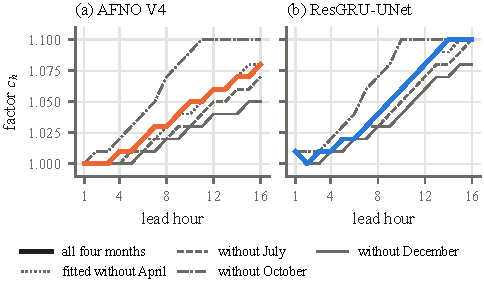
\includegraphics[width=0.55\textwidth]{fig_calib_scales.pdf}
\caption{Fitted calibration factors $c_h$ of the five-seed ensembles by lead hour: fitted on all four validation months (thick) and with one month left out (thin).}
\label{fig:calibscales}
\end{figure}

\begin{table}[!htbp]
\centering
\caption{Five-seed ensemble scores by validation month (no calibration)}
\label{tab:months}
\begin{tabular}{@{}lccc@{}}
\toprule
Month & AFNO V4 & ResGRU-UNet & Gap \\
\midrule
April & 0.9097 & 0.9162 & +0.0064 \\
July & 0.9056 & 0.9091 & +0.0035 \\
October & 0.9233 & 0.9271 & +0.0038 \\
December & 0.9194 & 0.9249 & +0.0055 \\
\bottomrule
\end{tabular}
\end{table}

\begin{table}[!htbp]
\centering
\caption{Five-seed ensembles by true concentration (\ugm): share of values, mean SMAPE and mean log bias (positive: too high)}
\label{tab:bins}
\setlength{\tabcolsep}{3pt}
\begin{tabular}{@{}lrcccc@{}}
\toprule
 & & \multicolumn{2}{c}{SMAPE} & \multicolumn{2}{c}{Log bias} \\
\cmidrule(lr){3-4}\cmidrule(l){5-6}
Bin & Share & AFNO & ResGRU & AFNO & ResGRU \\
\midrule
0 to 10 & 36.5\% & 0.261 & 0.241 & +0.103 & +0.085 \\
10 to 25 & 26.1\% & 0.181 & 0.167 & +0.071 & +0.050 \\
25 to 50 & 16.6\% & 0.177 & 0.161 & +0.073 & +0.048 \\
50 to 100 & 11.8\% & 0.158 & 0.144 & +0.070 & +0.046 \\
100 to 200 & 6.5\% & 0.160 & 0.149 & +0.046 & +0.021 \\
above 200 & 2.5\% & 0.147 & 0.147 & $-$0.009 & $-$0.026 \\
\bottomrule
\end{tabular}
\end{table}

\begin{table}[!htbp]
\centering
\caption{Training curves of the 12 logged runs (ResGRU: ResGRU-UNet; s: seed): best epoch and its validation score, the score at the last epoch (16), the drop, the lowest training loss, and the validation loss at a training loss of 0.09 (interpolated)}
\label{tab:curves}
\setlength{\tabcolsep}{2.4pt}
\begin{tabular}{@{}lcccccc@{}}
\toprule
Run & Peak & $S$ peak & $S$ last & Drop & Min tr. & Val@0.09 \\
\midrule
AFNO V4, s1 & 4 & 0.91178 & 0.90260 & 0.0092 & 0.0537 & 0.1247 \\
AFNO V4, s2 & 4 & 0.91227 & 0.90222 & 0.0101 & 0.0536 & 0.1241 \\
AFNO V4, s3 & 5 & 0.91080 & 0.90185 & 0.0090 & 0.0539 & 0.1257 \\
ResGRU, s42 & 7 & 0.91579 & 0.91237 & 0.0034 & 0.0660 & 0.1178 \\
ResGRU, s1337 & 6 & 0.91523 & 0.91222 & 0.0030 & 0.0646 & 0.1174 \\
ResGRU, s1 & 7 & 0.91687 & 0.91273 & 0.0041 & 0.0679 & 0.1168 \\
ResGRU, s2 & 6 & 0.91784 & 0.91337 & 0.0045 & 0.0635 & 0.1146 \\
ResGRU, s3 & 7 & 0.91578 & 0.91294 & 0.0028 & 0.0679 & 0.1180 \\
AFNO V4, H1 & 4 & 0.91259 & 0.90342 & 0.0092 & 0.0534 & 0.1236 \\
AFNO V4, H2 & 4 & 0.91062 & 0.90161 & 0.0090 & 0.0542 & 0.1257 \\
AFNO V4, H3 & 4 & 0.91094 & 0.90150 & 0.0094 & 0.0539 & 0.1255 \\
ResGRU, H4 & 7 & 0.91456 & 0.90988 & 0.0047 & 0.0651 & 0.1202 \\
\bottomrule
\end{tabular}
\end{table}

\begin{table}[!htbp]
\centering
\caption{Ridge penalty search on validation}
\label{tab:ridgegrid}
\begin{tabular}{@{}lc@{}}
\toprule
Penalty $\lambda$ & Validation $S$ \\
\midrule
$10^{-2}$ & 0.86370 \\
$10^{0}$ & 0.86370 \\
$10^{2}$ & 0.86368 \\
$10^{4}$ & 0.86227 \\
$10^{6}$ & 0.85753 \\
0 (persistence) & 0.85154 \\
\bottomrule
\end{tabular}
\end{table}

\subsection{Regression Metrics}
Table~\ref{tab:regfull} gives the validation metrics of every model on the raw scale and in $\log(1+y)$, with the Pearson correlation $r$ over all values. The log-space $R^2$ orders the finalists as the raw one does (0.952 against 0.944 for the five-seed ensembles).

\begin{table}[!htbp]
\centering
\caption{Validation metrics of every model: raw scale (MAE, RMSE in \ugm), log space, pooled correlation $r$, skill (\%) and benchmark score $S$}
\label{tab:regfull}
\begin{tabular}{@{}lrrrrrrrrr@{}}
\toprule
 & \multicolumn{3}{c}{Raw scale} & \multicolumn{3}{c}{$\log(1+y)$} & & & \\
\cmidrule(lr){2-4}\cmidrule(lr){5-7}
Model & MAE & RMSE & $R^2$ & MAE & RMSE & $R^2$ & $r$ & Skill & $S$ \\
\midrule
Persistence & 10.44 & 26.46 & 0.767 & 0.268 & 0.404 & 0.895 & 0.884 & 0.0 & 0.8515 \\
Seasonal naive & 11.53 & 26.80 & 0.761 & 0.358 & 0.511 & 0.832 & 0.877 & $-$1.3 & 0.7907 \\
Ridge & 8.51 & 21.48 & 0.847 & 0.234 & 0.347 & 0.923 & 0.924 & 18.8 & 0.8637 \\
\midrule
ResGRU-UNet, seed 42 & 6.57 & 18.57 & 0.885 & 0.176 & 0.282 & 0.949 & 0.948 & 29.8 & 0.9158 \\
AFNO V4, seed 42 & 7.31 & 20.17 & 0.865 & 0.192 & 0.304 & 0.941 & 0.944 & 23.8 & 0.9110 \\
FMG-WACLU, seed 42 & 7.14 & 19.32 & 0.876 & 0.190 & 0.299 & 0.942 & 0.943 & 27.0 & 0.9099 \\
patch AFNO, seed 42 & 6.85 & 19.02 & 0.880 & 0.188 & 0.299 & 0.943 & 0.944 & 28.1 & 0.9031 \\
ConvLSTM, seed 42 & 7.05 & 18.93 & 0.881 & 0.195 & 0.306 & 0.940 & 0.939 & 28.5 & 0.8945 \\
\midrule
AFNO V4, seed 1337 & 7.26 & 19.88 & 0.869 & 0.192 & 0.303 & 0.941 & 0.944 & 24.9 & 0.9114 \\
AFNO V4, seed 1 & 7.24 & 20.10 & 0.866 & 0.190 & 0.302 & 0.941 & 0.944 & 24.0 & 0.9118 \\
AFNO V4, seed 2 & 7.23 & 19.74 & 0.870 & 0.191 & 0.303 & 0.941 & 0.945 & 25.4 & 0.9123 \\
AFNO V4, seed 3 & 7.06 & 19.72 & 0.871 & 0.186 & 0.296 & 0.944 & 0.945 & 25.5 & 0.9108 \\
ResGRU-UNet, seed 1337 & 6.56 & 18.57 & 0.885 & 0.174 & 0.277 & 0.951 & 0.949 & 29.8 & 0.9152 \\
ResGRU-UNet, seed 1 & 6.58 & 18.53 & 0.886 & 0.176 & 0.285 & 0.948 & 0.948 & 30.0 & 0.9169 \\
ResGRU-UNet, seed 2 & 6.51 & 18.49 & 0.886 & 0.173 & 0.274 & 0.952 & 0.950 & 30.1 & 0.9178 \\
ResGRU-UNet, seed 3 & 6.65 & 18.80 & 0.882 & 0.178 & 0.286 & 0.948 & 0.948 & 28.9 & 0.9158 \\
\midrule
AFNO V4, H1 & 7.03 & 19.51 & 0.873 & 0.187 & 0.299 & 0.943 & 0.945 & 26.2 & 0.9126 \\
AFNO V4, H2 & 7.13 & 19.71 & 0.871 & 0.189 & 0.302 & 0.942 & 0.944 & 25.5 & 0.9106 \\
AFNO V4, H3 & 7.31 & 20.33 & 0.863 & 0.191 & 0.303 & 0.941 & 0.943 & 23.1 & 0.9109 \\
ResGRU-UNet, H4 & 6.70 & 18.85 & 0.882 & 0.180 & 0.289 & 0.946 & 0.947 & 28.8 & 0.9146 \\
\midrule
AFNO V4, 2 seeds & 7.15 & 19.73 & 0.871 & 0.188 & 0.300 & 0.942 & 0.946 & 25.4 & 0.9131 \\
\ + cal., in sample & 7.84 & 21.28 & 0.849 & 0.199 & 0.314 & 0.937 & 0.944 & 19.6 & 0.9143 \\
\ + cal., one month out & 7.90 & 21.13 & 0.852 & 0.201 & 0.316 & 0.936 & 0.943 & 20.1 & 0.9134 \\
AFNO V4, 5 seeds & 6.99 & 19.45 & 0.874 & 0.184 & 0.296 & 0.944 & 0.947 & 26.5 & 0.9145 \\
\ + cal., in sample & 7.69 & 21.02 & 0.853 & 0.196 & 0.310 & 0.938 & 0.945 & 20.6 & 0.9158 \\
\ + cal., one month out & 7.76 & 20.90 & 0.855 & 0.197 & 0.311 & 0.938 & 0.945 & 21.0 & 0.9149 \\
\midrule
ResGRU-UNet, 2 seeds & 6.40 & 18.21 & 0.890 & 0.171 & 0.274 & 0.952 & 0.950 & 31.2 & 0.9175 \\
\ + cal., in sample & 7.22 & 20.17 & 0.865 & 0.184 & 0.292 & 0.945 & 0.948 & 23.8 & 0.9198 \\
\ + cal., one month out & 7.23 & 20.00 & 0.867 & 0.185 & 0.292 & 0.945 & 0.948 & 24.4 & 0.9193 \\
ResGRU-UNet, 5 seeds & 6.32 & 18.04 & 0.892 & 0.169 & 0.273 & 0.952 & 0.951 & 31.8 & 0.9193 \\
\ + cal., in sample & 7.13 & 19.94 & 0.868 & 0.182 & 0.290 & 0.946 & 0.949 & 24.6 & 0.9215 \\
\ + cal., one month out & 7.12 & 19.71 & 0.871 & 0.183 & 0.290 & 0.946 & 0.949 & 25.5 & 0.9210 \\
\bottomrule
\end{tabular}
\end{table}

\begin{table}[!tp]
\centering
\caption{Every test score of the study (UTC date of scoring; the description as recorded at submission)}
\label{tab:tests}
\small
\begin{tabular}{@{}l>{\raggedright\arraybackslash}p{0.66\textwidth}cc@{}}
\toprule
Date & Forecast & Public & Private (test) \\
\midrule
2026-11-07 & ablation: AFNO V4 seed 1337 only, no calibration & 0.8882 & 0.8749 \\
2026-11-07 & ablation: AFNO V4 seed 42 only, no calibration & 0.8878 & 0.8762 \\
2026-11-07 & ablation: AFNO V4 2-seed mean, no calibration & 0.8899 & 0.8779 \\
2026-11-07 & ResGRU-UNet in the V4 pipeline, seed 42, val 0.9158 & 0.8924 & 0.8798 \\
2026-11-07 & ConvLSTM in the V4 pipeline, seed 42, val 0.8945 & 0.8537 & 0.8452 \\
2026-11-07 & FMG-WACLU in the V4 pipeline, seed 42, val 0.9099 & 0.8862 & 0.8710 \\
2026-11-07 & patch AFNO, bug fixed in the V4 pipeline, seed 42, val 0.9031 & 0.8680 & 0.8530 \\
2026-11-07 & final: ResGRU-UNet 2 seeds (42$+$1337) mean, no calibration, val 0.9175 & 0.8948 & 0.8817 \\
2026-11-07 & final: ResGRU-UNet 2 seeds $+$ V4 per-horizon calibration (full V4 recipe) & 0.9033 & 0.8898 \\
2026-11-08 & 5 seeds: AFNO V4 5-seed mean $+$ V4 per-horizon calibration, val 0.9158 (in sample) & 0.8972 & 0.8848 \\
2026-11-08 & 5 seeds: ResGRU-UNet 5-seed mean $+$ V4 per-horizon calibration, val 0.9215 (in sample) & 0.9056 & 0.8914 \\
2026-11-08 & 5 seeds: AFNO V4 5-seed mean, no calibration, val 0.9145 & 0.8911 & 0.8793 \\
2026-11-08 & 5 seeds: ResGRU-UNet 5-seed mean, no calibration, val 0.9193 & 0.8975 & 0.8838 \\
2026-11-08 & 5 seeds: ResGRU-UNet seed 1337 only, no calibration, val 0.9152 & 0.8930 & 0.8788 \\
2026-11-08 & 5 seeds: AFNO V4 seed 1 only, no calibration, val 0.9118 & 0.8881 & 0.8758 \\
2026-11-08 & 5 seeds: ResGRU-UNet seed 1 only, no calibration, val 0.9169 & 0.8956 & 0.8796 \\
2026-11-08 & 5 seeds: AFNO V4 seed 2 only, no calibration, val 0.9123 & 0.8880 & 0.8767 \\
2026-11-08 & 5 seeds: AFNO V4 seed 3 only, no calibration, val 0.9108 & 0.8876 & 0.8734 \\
2026-11-08 & 5 seeds: ResGRU-UNet seed 2 only, no calibration, val 0.9178 & 0.8951 & 0.8805 \\
2026-11-08 & 5 seeds: ResGRU-UNet seed 3 only, no calibration, val 0.9158 & 0.8957 & 0.8810 \\
2026-11-08 & ablation H1: AFNO V4 with all-hour skips, seed 42, no calibration, val 0.9126 & 0.8865 & 0.8748 \\
2026-11-08 & ablation H3: AFNO V4 with soft-threshold 0, seed 42, no calibration, val 0.9109 & 0.8868 & 0.8758 \\
2026-11-08 & ablation H2: AFNO V4 with zero-padded AFNO blocks, seed 42, no calibration, val 0.9106 & 0.8869 & 0.8745 \\
2026-11-08 & ablation H4: ResGRU-UNet without ConvGRU recurrence, seed 42, no calibration, val 0.9146 & 0.8944 & 0.8798 \\
2026-11-08 & baseline: persistence (last input hour repeated for 16 h), no model, val 0.8515 & 0.8024 & 0.7910 \\
2026-11-08 & baseline: ridge regression (20 channels last hour $+$ PM history), val 0.8637 & 0.8071 & 0.7951 \\
2026-11-16 & post hoc: ResGRU-UNet 5-seed mean $+$ LightGBM correction fitted on all 4 val months, no calibration, out-of-fold val 0.9051 (rule verdict: no gain) & 0.8775 & 0.8608 \\
\bottomrule
\end{tabular}
\end{table}

\subsection{Every Test Score}
Table~\ref{tab:tests} lists every forecast of the study that was scored on the test set, with the scores of both parts. The first three rows score V4's own forecasts, so that the study's numbers for AFNO V4 come from the same server as the rest. Wherever both finalists have a score at the same setting, the public and private parts order them the same way.

\subsection{Automated Checks}
Each analysis stage writes its checks into its run record, and the record is kept only if they pass. Table~\ref{tab:checks} counts them; all 68 pass. They fall into four kinds: recomputed scores equal the logged ones (for example, each seed's validation score, the five-seed ensembles and the two-seed calibration); test forecasts equal the training run's own output (relative difference below $10^{-3}$); identities that must hold (zero ridge weights give persistence; a zero hybrid correction gives the ensemble; the truth scored against itself gives MAE 0, RMSE 0 and $R^2$ 1); and data checks (shapes, finite and non-negative forecasts, no month fitted on itself).

\begin{table}[!htbp]
\centering
\caption{Automated checks in the run records}
\label{tab:checks}
\setlength{\tabcolsep}{3pt}
\begin{tabular}{@{}lrp{0.55\columnwidth}@{}}
\toprule
Stage & Checks & Examples \\
\midrule
Final round & 7 & seed scores equal the logs; V4 test forecasts and calibration factors reproduced \\
Analysis & 16 & ten seeds' validation scores; six seeds' test forecasts \\
Regression & 29 & 17 runs, the ensembles and calibration, persistence, truth against itself \\
Baselines & 3 & 24-h lag inside the month; loader truth equals the raw series \\
Ridge & 3 & zero weights give persistence; valid test forecasts \\
Hybrid & 8 & zero correction gives the ensemble, on validation and test; out-of-fold folds \\
Maps & 2 & map shapes; maps average to the regression MAE \\
\midrule
Total & 68 & all pass \\
\bottomrule
\end{tabular}
\end{table}

\subsection{Additional Results}
Table~\ref{tab:deciles} splits the SMAPE of the two ensembles by how polluted a cell is, Fig.~\ref{fig:terms} splits the score into its three terms by lead hour, Fig.~\ref{fig:case} shows one window in detail, and Fig.~\ref{fig:smape} maps the SMAPE of both ensembles.

\begin{table}[!htbp]
\centering
\caption{Mean SMAPE of the five-seed ensembles in each decile of cells, ranked by mean \PM{} (\ugm)}
\label{tab:deciles}
\setlength{\tabcolsep}{3pt}
\begin{tabular}{@{}clccc@{}}
\toprule
Decile & Cell mean & AFNO V4 & ResGRU-UNet & Difference \\
\midrule
1 & 3.0 to 5.4 & 0.231 & 0.213 & $-$0.017 \\
2 & 5.4 to 10.4 & 0.264 & 0.245 & $-$0.019 \\
3 & 10.4 to 13.9 & 0.198 & 0.186 & $-$0.012 \\
4 & 13.9 to 17.4 & 0.193 & 0.180 & $-$0.013 \\
5 & 17.4 to 24.1 & 0.218 & 0.199 & $-$0.019 \\
6 & 24.1 to 35.5 & 0.188 & 0.170 & $-$0.017 \\
7 & 35.5 to 45.0 & 0.160 & 0.147 & $-$0.013 \\
8 & 45.0 to 61.2 & 0.180 & 0.167 & $-$0.013 \\
9 & 61.2 to 82.7 & 0.179 & 0.163 & $-$0.016 \\
10 & 82.7 to 294.5 & 0.236 & 0.217 & $-$0.019 \\
\bottomrule
\end{tabular}
\end{table}

\begin{figure}[!htbp]
\centering
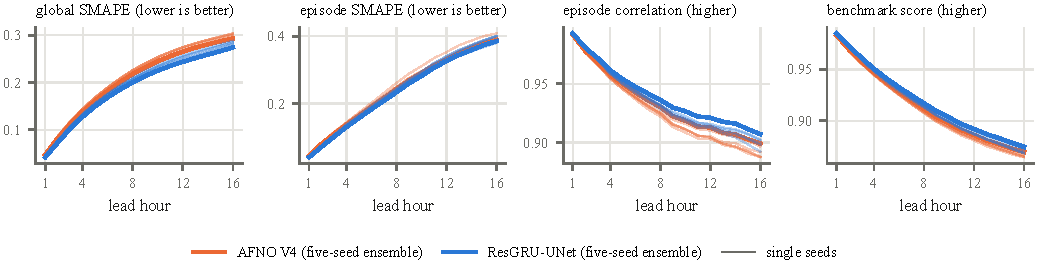
\includegraphics[width=0.85\textwidth]{fig_terms_by_hour.pdf}
\caption{The three terms of the benchmark score and the score itself by lead hour, on validation. Thin lines: single seeds; thick lines: five-seed means.}
\label{fig:terms}
\end{figure}

\begin{figure}[!htbp]
\centering
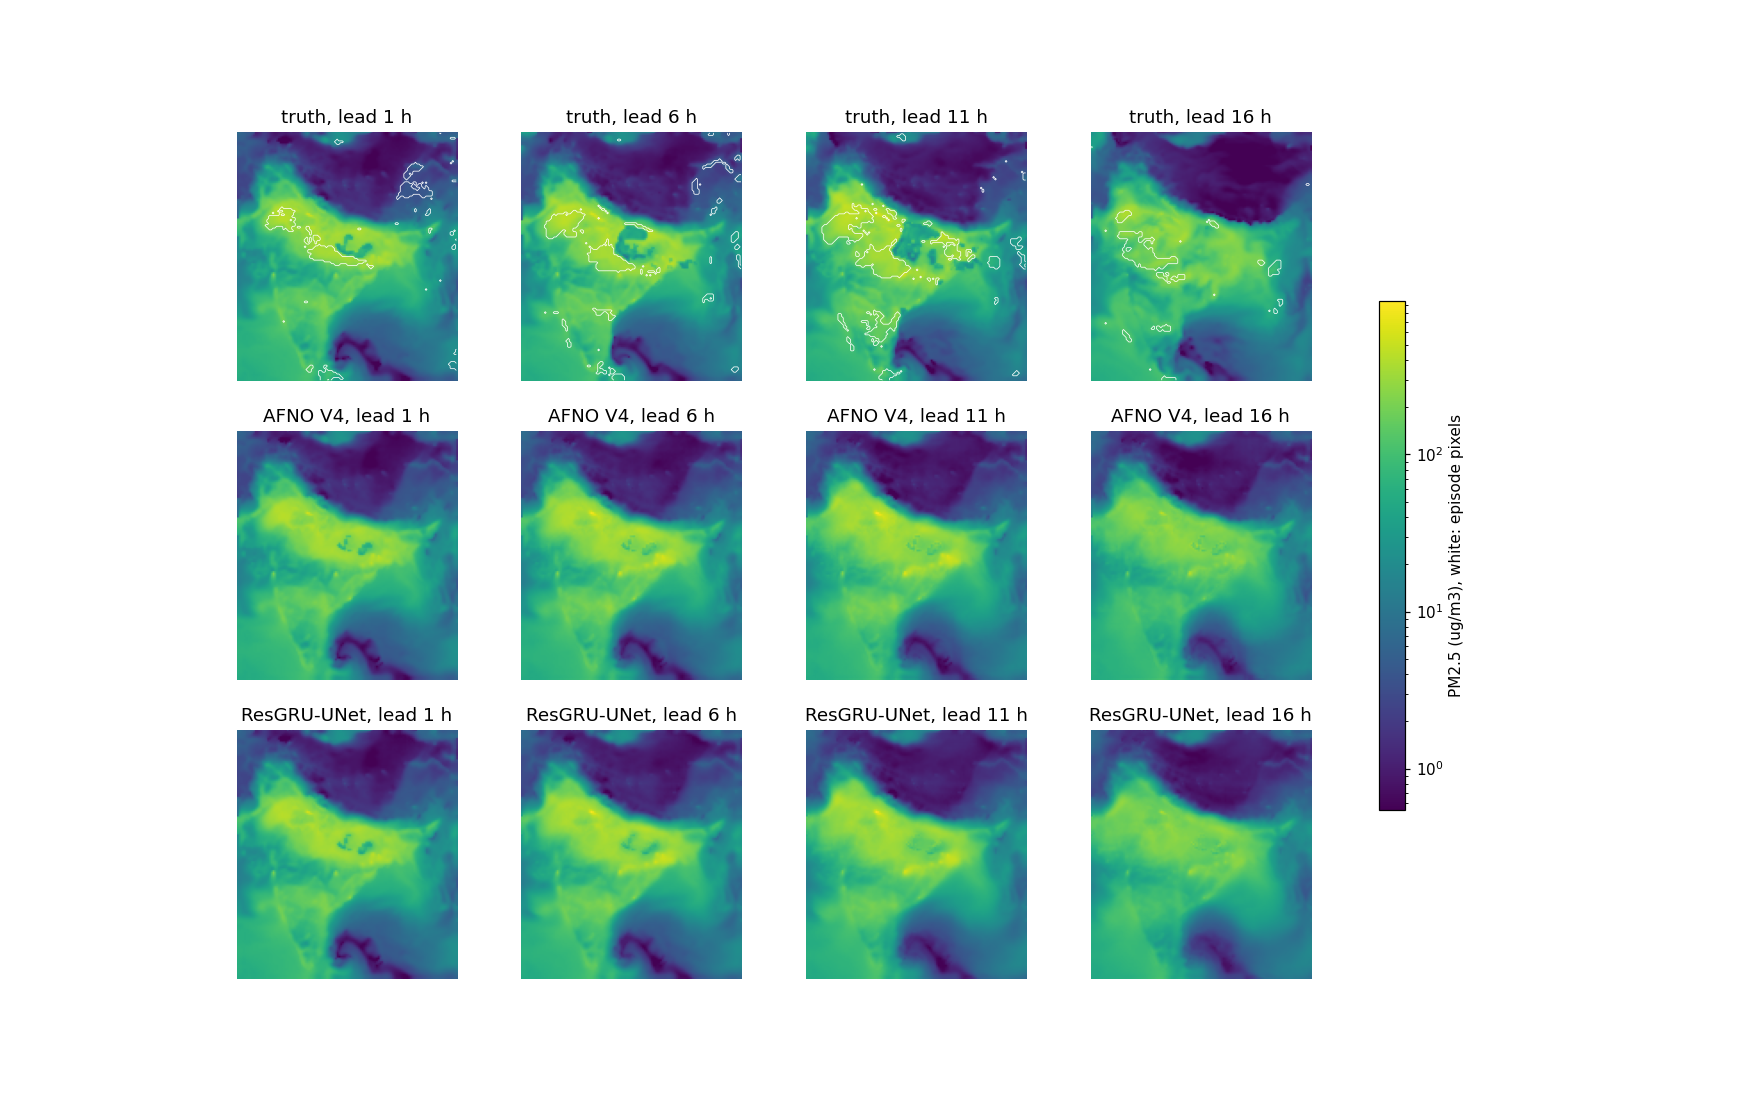
\includegraphics[width=0.5\textwidth, trim=155 79 194 71, clip]{fig_case.png}
\caption{The validation window with the most episode cells (December): truth with episode cells outlined (top), AFNO V4 (middle) and ResGRU-UNet (bottom) at lead hours 1, 6, 11 and 16, in grid coordinates on a log colour scale. Both smooth the episode structure; ResGRU-UNet scores higher on this window (0.9116 against 0.9103) but has the lower episode correlation (0.928 against 0.944).}
\label{fig:case}
\end{figure}

\begin{figure}[!htbp]
\centering
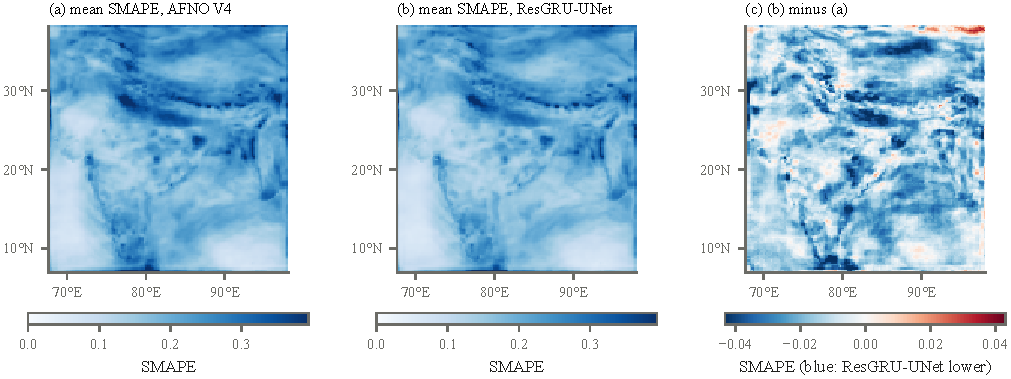
\includegraphics[width=0.85\textwidth]{fig_smape_maps.pdf}
\caption{Mean SMAPE per cell for the five-seed means of AFNO V4 (a) and ResGRU-UNet (b), and their difference (c). ResGRU-UNet is lower in 94.7\% of cells.}
\label{fig:smape}
\end{figure}
\FloatBarrier
\end{document}
